% ------------------------------------------------------------------------
% ------------------------------------------------------------------------
% ICMC: Modelo de Trabalho Acadêmico (tese de doutorado, dissertação de
% mestrado e trabalhos monográficos em geral) em conformidade com 
% ABNT NBR 14724:2011: Informação e documentação - Trabalhos acadêmicos -
% Apresentação
% ------------------------------------------------------------------------
% ------------------------------------------------------------------------

% Opções: 
%   Qualificação          = qualificacao 
%   Curso                 = doutorado/mestrado
%   Situação do trabalho  = pre-defesa/pos-defesa (exceto para qualificação)
%   Versão para impressão = impressao
\documentclass[qualificacao, mestrado]{packages/icmc}

% ---------------------------------------------------------------------------
% Pacotes Opcionais
% ---------------------------------------------------------------------------
\usepackage{rotating}           % Usado para rotacionar o texto
\usepackage[all,knot,arc,import,poly]{xy}   % Pacote para desenhos gráficos
% Este pacote pode conflitar com outros pacotes gráficos como o ``pictex''
% Então é necessário usar apenas um dos pacotes conflitantes
\newcommand{\VerbL}{0.52\textwidth}
\newcommand{\LatL}{0.42\textwidth}
% ---------------------------------------------------------------------------
%\usepackage{eucal}
%\usepackage[mathcal]{eucal}
\usepackage[mathscr]{eucal}
\usepackage{tikz}
\usetikzlibrary{quotes, angles, intersections}


\floatname{algorithm}{Procedure}
\renewcommand{\algorithmicrequire}{\textbf{Input:}}
\renewcommand{\algorithmicensure}{\textbf{Output:}}

%\usepackage{algorithm2e}

%MEUS COMANDOs
\newcommand{\R}{\mathbb{R}}
\newcommand{\D}{\mathscr{D}}
\newcommand{\Pp}{\mathscr{P}}
\newcommand{\Cc}{\mathscr{C}}
\newcommand{\E}{\mathscr{E}}



\newcommand{\bigO}{\mathscr{O}}
%\newcommand{\fautor}{\legend{Reference: Made by the author.}}


%siglas
\newcommand{\MCLP}{MCLP}
\newcommand{\PMCLP}{PMCLP}


%FIM MEUS COMANDOS

% ---
% Informações de dados para CAPA e FOLHA DE ROSTO
% ---
% Tanto na capa quanto nas folhas de rosto apenas a primeira letra da primeira palavra (ou nomes próprios) devem estar em letra maiúscula, todas as demais devem ser em letra minúscula.
\tituloPT{Cobertura Planar Maximal por Elipses}
\tituloEN{Planar Maximal Covering with Ellipses}
\autor[Tedeschi, D. F.]{Danilo Françoso Tedeschi}
\genero{M} % Gênero do autor (M = Masculino / F = Feminino)
\orientador[Orientadora]{Profa. Dra.}{Marina Andretta}
%\coorientador{Prof. Dr.}{Fulano de Tal}
\curso{CCMC}
\data{01}{03}{2019} % Data do depósito
\idioma{EN} % Idioma principal do documento (PT = português / EN = inglês)
% ---


% ---
% RESUMOS
% ---

% Resumo em PORTUGUÊS
% conter no máximo 500 palavras
% conter no mínimo 1 e no máximo 5 palavras-chave
%\textoresumo[brazil]{
 %   Este trabalho é um breve modelo  para a escrita de monografias de qualificação, dissertações e teses utilizando o ambiente \LaTeX, de acordo com as normas exigidas pelo Instituto de Ciências Matemáticas e de Computação (ICMC), da Universidade de São Paulo (USP). Para a confecção deste modelo foi utilizado a última versão (1.9.6) do pacote de classes \textit{abnTeX2} que segue as normas da Associação Brasileira de Normas Técnicas. A elaboração de uma monografia, dissertação ou tese pode ser feita sobrescrevendo o conteúdo deste modelo. 
 %   }{Modelo, Monografia de qualificação, Dissertação, Tese, Latex}


% resumo em INGLÊS
% conter no máximo 500 palavras
% conter no mínimo 1 e no máximo 5 palavras-chave
\textoresumo[english]{
    Planar maximal covering with ellipses is an optimization problem where one wants to place ellipses on the plane to cover demand points, such that a function depending on the value of the covered points and on the cost of the ellipses that have been used is maximized. Initially, we developed an algorithm for the version of the problem where the ellipses are parallel to the coordinate axis. For the future, we intend to adapt an approximation algorithm developed for the planar maximal covering by disks and develop a method for the variant of the problem where the ellipses can be freely rotated. 
    }{Optimization, Planar Maximal Covering Location Problem, maximal covering of points using ellipses}

% ----------------------------------------------------------
% ELEMENTOS PRÉ-TEXTUAIS
% ----------------------------------------------------------

% Inserir a ficha catalográfica
%\incluifichacatalografica{tex/pre-textual/ficha-catalografica.pdf}

% DEDICATÓRIA / AGRADECIMENTO / EPÍGRAFE
%\textodedicatoria*{tex/pre-textual/dedicatoria}
%\textoagradecimentos*{tex/pre-textual/agradecimentos}
%\textoepigrafe*{tex/pre-textual/epigrafe}

% Inclui a lista de figuras
\incluilistadefiguras

% Inclui a lista de tabelas
%\incluilistadetabelas

% Inclui a lista de quadros
%\incluilistadequadros

% Inclui a lista de algoritmos
\incluilistadealgoritmos

% Inclui a lista de códigos
%\incluilistadecodigos

% Inclui a lista de siglas e abreviaturas
%\incluilistadesiglas

% Inclui a lista de símbolos
%\incluilistadesimbolos

% ----
% Início do documento
% ----
\begin{document}
% ----------------------------------------------------------
% ELEMENTOS TEXTUAIS
% ----------------------------------------------------------
\textual

\chapter{Introduction}
\label{chapter:introduction}
Two main types of optimal covering problems can be found in the literature: the Minimum Cover Problem, also known as just Set Cover Problem, and the Maximal Covering Problem \cite{karatas}. 

One of the 21 Karp's NP-Complete problems\footnote{The decision version, which asks if there is a cover of size $k$, is NP-Complete.} \cite{karp}, the Minimum Cover Problem is very well explored and considered to be a classic. 
Given a demand set and collection of subsets of the demand set, the problem asks what is the minimum number of elements from the collection of subsets needed to cover the whole demand set. One of its most famous examples is the Minimum Vertex Cover defined over graphs, where the vertex set has to be covered by a subset of edges.

The second type of covering problems arose from the fact that covering almost all the demand set can be a lot cheaper than having to cover it all \cite{garcia}. This second type is known as \sigla{\MCLP}{Maximal Covering Location Problem} and was introduced in \cite{church:1974}. In this first study, it is defined on a network with demand nodes, a facility set is also given and a solution maximizes the demand coverage satisfying the constraint that only a subset of the facilities is used. Just like the Minimum Cover, MCLP is a NP-Hard problem \cite{hatta:2013} and both deterministic, (using integer programming) \cite{church:1974}, and heuristic methods \cite{revelle:2008} have been proposed to solve it.

In \cite{church:1984} a new kind of MCLP named \sigla{\PMCLP}{Planar Maximal Covering Location Problem} was introduced. This version of the problem was not defined on a network, instead the demand set and the facilities are located in $\R^2$ having the coverage area of a facility be defined by a distance function. PMCLP is said to have been studied under Euclidean and rectilinear distance functions \cite{younies}. The Euclidean norm PMCLP, which has a lot of results that can be applied for the elliptical PMCLP, is also found in the literature as the problem of maximization of points covered by a fixed number of unit disks \cite{cabello:2006}. 
Early works only tackled the one-disk version of the problem, in \cite{chazelle:1986} a $\bigO(n^2)$ algorithm, which still stands as the best in terms of run-time complexity, was proposed besting the prior $\bigO(n^2\log{n})$ algorithm created by \cite{drezner}.
The $m$ unit disks maximal covering was studied in \cite{cabello:2006} which had as its most important result a $(1-\epsilon)$-approximation algorithm which runs in $\bigO(n\log{n})$. To achieve its main goal, however, they developed a deterministic $\bigO(n^{2m-1}\log{n})$ algorithm which gets employed into their approximation scheme.
Additionally, in \cite{aronov:2008} one-disk maximal covering is proven to be 3SUM-HARD. This means that maximizing the amount of points covered by a disk is as hard as finding three real numbers that sum to zero among $n$ given real numbers.

Planar maximal covering with ellipses differs from its disks counterpart only in the shape of the facility's coverage area. The main motivation to study this modified version is that cellphone towers can have elliptical shaped coverage area, so in order to determine what are the best locations to place $m$ cellphone towers to maximize the amount of the population covered by its signal, an elliptical PMCLP is better suited \cite{canbolat}. Only two articles have been found published in the literature that study this problem. In \cite{canbolat}, a mixed non-linear programming method was proposed as a first approach to the problem. For some instances the method took too long and did not find the optimal solution. For this reason a heuristic method was developed using a technique called Simulated Annealing, solutions for the instances that timed-out with the first method were then obtained. The problem was further explored in \cite{andreta} which proposed a deterministic method that showed better performance obtaining the optimal solutions for the instances which the first method could not. Also, in \cite{andreta}, a version of the problem where every ellipse can be freely rotated was introduced and an exact method, which could not find the optimal solutions for large instances, and a heuristic method were proposed for it. Despite the similarities, none of the works cited above base their development on the maximal covering with disks algorithms found in the literature.


This work is structured in the following way: \autoref{chapter:definitions} introduces some definitions and results that are used throughout the next chapters; in \autoref{chapter:pmclp}, the maximal covering by disks problem is studied and a $\bigO(n^{2m})$ algorithm is proposed; in \autoref{chapter:ellipses}, the maximal covering by ellipses is introduced and the algorithm for the disks case is adapted for it; finally, \autoref{chapter:future_work} presents what is left as future work. Also, \autoref{chapter:ellipses_intersection} determines with detail the intersection of two ellipses, which is used in the algorithm developed in \autoref{chapter:ellipses}.



\chapter{Notation and Preliminaries}
\label{chapter:definitions}
Some definitions and results that are used throughout the text are given in this chapter.

\section{Norm}

A norm is a function that maps every vector from a vector space onto a non-negative real number satisfying some conditions. Here it is defined for the vector space $\R^2$ as follows

\begin{definicao}
Let $\xi : \R^2 \mapsto [0, \infty]$, $\xi$ is said to be a norm function of $\R^2$ if for any $p, q \in \R^2$ and $a \in \R$,

\begin{enumerate}
    \item $\xi(p + q) \le \xi(p) + \xi(q)$
    \item $\xi(ap) = |a|\xi(p)$
    \item if $\xi(p)=0$, then $p=0$
\end{enumerate}

\end{definicao}

\subsection{Elliptical and euclidean norm functions}

Let $u \in \R^2$ be a vector, the euclidean norm of $u$ is defined as

\begin{equation}\label{eq:norm2}
||u||_2 = \sqrt{u^{T}u}
\end{equation}

The elliptical norm takes a $2$ by $2$ positive definite matrix as its parameter. This matrix can be seen as a linear transformation of the euclidean norm. Let $u \in \R^2$ be a vector and $Q$ be a $2$ by $2$ positive definite matrix, the elliptical norm of $u$ is defined as 

\begin{equation}
||u||_{elliptical} = \sqrt{u^{T}Qu}
\end{equation}

It is easy to see that the elliptical norm, when taking $Q$ to be the identity matrix, becomes the euclidean norm.

Determining the distance between two points, given a norm function is done by calculating the norm of the vector defined by the difference between the two points. For example, the elliptical distance between the points $p,q \in \R^2$ is given by $||p-q||_{elliptical}$.

\section{Disk}

A circle (or circumference) is a set of points in $\R^2$ that have constant euclidean distance, also known as radius, to another point, also referred to as the center of the circle. A unit circle is a circle with radius equal to $1$.
A disk is the set of points bounded by a circle, in other words let $c \in \R^2$, a unit disk with center $c$ is the set of every point $p \in \R^2$ which satisfy \autoref{eq:disk}.

\begin{equation}\label{eq:disk}
||p-c||_2^2 \le 1
\end{equation} 

\section{Ellipse}

The ellipse is a curve which is categorized, along with the parabola and the hyperbola, as a conic section. As the name suggests, conic sections are curves resulted from the intersection of a right circular cone in $\R^3$ with a plane \cite{brannan:geometry}. From that definition, an equation which describes any conic section is given as follows

\begin{equation}\label{equation:quadratic_form}
Ax^2 + Bxy + Cy^2 + Dx + Ey + F = 0
\end{equation}

To distinguish an ellipse from the other conic sections given an instance of \autoref{equation:quadratic_form}, the condition $4AC - B^2>0$ can be verified \cite{ayoub}.

Assuming the center of an ellipse is $c \in \R^2$, then \autoref{equation:quadratic_form} can be rewritten as a quadratic form as follows

\begin{equation}
(p-c)^{T}Q(p-c) = 1
\end{equation}

with $p \in \R^2$ and $Q$ being a $2$ by $2$ positive definite matrix which carries the parameters of the ellipse. From \autoref{equation:quadratic_form}, $Q$ can be defined as follows

\[
Q=
\left( {\begin{array}{cc}
	A & \frac{B}{2} \\
	\frac{B}{2} & C \\
	\end{array} } \right).
\]

Note that asking $Q$ to be positive definite is the same as asking $4AC-B^2$ to be positive. This makes us arrive at the following definition of the ellipse

\begin{definicao}\label{def:ellipse}
    Let $c\in \R^2$ be the center of an ellipse and $Q$ be a $2$ by $2$ positive definite matrix, an ellipse is the set of every point $p \in \R^2$ that have $||p-c||_{elliptical}^2 = (p-c)^{T}Q(p-c) = 1$. Also, a point $p$ is considered covered by an ellipse if $||p-c||_{elliptical}^2 = (p-c)^{T}Q(p-c) \le 1$.
\end{definicao}

An alternative way to define an ellipse, which can be seen as just a property derived from the definition above, is to begin its construction with two points called foci and a constant $R \in \R$, with $R$ being greater than the euclidean distance between the two foci points (see \autoref{fig:ellipse_with_foci}). The ellipse is, then, defined as the set of points whose distance to the foci is equal to $R$. In other words, let $f_1, f_2 \in \R^2$ be the two foci points, the ellipse is the set of every point $p \in \R^2$, such that $||p-f_1||_2 + ||p-f_2||_2 = R$. It can be shown that this definition is equivalent to \autoref{def:ellipse}, with the coverage of a point $p$ being equivalent to $||p-f_1||_2 + ||p-f_2||_2 \le R$.

\begin{figure}[H]
    \centering
    
    \caption{A non-axis-parallel ellipse and its foci points.}
    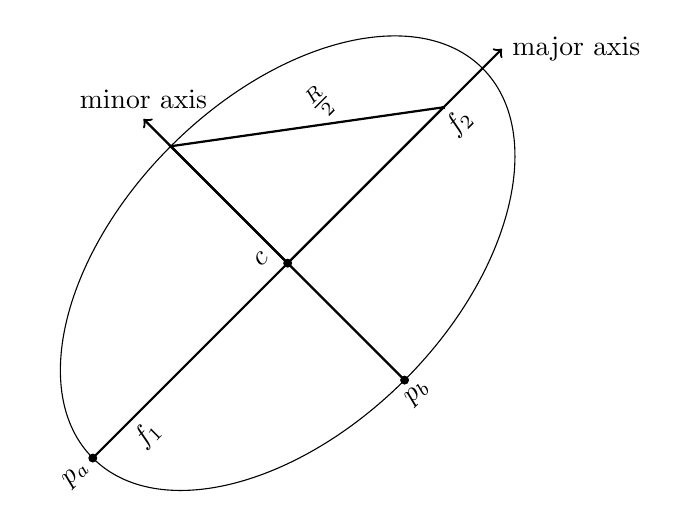
\begin{tikzpicture}[xscale=0.7, yscale=0.7][domain=0:11]
   % \draw [help axis] (-5,-3) grid (5,3);

    \begin{scope}[rotate=45]
    \draw (0,0) ellipse (5cm and 3cm);
    \node[rotate=45][below] at (-4,0) {$f_1$};
    \node[rotate=45][below] at (4,0) {$f_2$};
    \draw[fill] (-4,0) circle [radius=.5pt];
    \draw[fill] (4,0) circle [radius=.5pt];
    \draw [thick] (4,0) -- (0,0) -- (0,3) -- (4,0);
    \draw[->,thick] (-5,0)--(5.5,0) node[right]{major axis};
    \draw[->,thick] (0,-3)--(0,3.7) node[above]{minor axis};
        \node[rotate=45] [left] at (0,0.4) {$c$};
    \node [rotate=45][right] at (2.1,1.65) {$\frac{R}{2}$};
    
   
    \node [rotate=45][left] at (-5,0) {$p_a$};
    \draw[fill] (-5,0) circle [radius=2pt];
    
        \draw[fill] (0,0) circle [radius=2pt];
    
    \draw[fill] (0,-3) circle [radius=2pt];
    \node [below][rotate=45] at (0,-3) {$p_b$};
    \end{scope}

    %a^2-b^2=c^2 -> c^2=25-9=16 -> c=4
    
    %\draw[fill] (0,0) circle [radius=.5pt];
	
    %
    %\draw[fill] (5,0) circle [radius=1pt];
    %\draw[fill] (0,3) circle [radius=1pt];
    %
    

    %\node [below] at (2.1,0) {$c$};
	%\node [left] at (-0.1,1.5) {$b$};



    %\node [above] at (5,0) {$(x_0+a,y_0)$};
    %\node [above] at (-5,0) {$(x_0-a,y_0)$};
    %\node [above] at (0,3) {$(x_0,y_0+b)$};
    %
    

    
    %\draw [-] (-5,0) -- (5,0);
     %\draw [-] (0,-3) -- (0,3);
     %\draw [|-|] (0.001,-0.1) -- (4.999,-0.1);
\end{tikzpicture}
    \fautor
    \label{fig:ellipse_with_foci}
\end{figure}

Also, in \autoref{fig:ellipse_with_foci}, the distance $a = ||p_a - c||_2$ is called the semi-major, and the distance $b = ||p_b-c||_2$ is called the semi-minor. These two values are also referred to as the shape parameters of an ellipse. Let $d = ||c-f_1||_2$, then it is easy to see that $a = R - d$ and $b = \sqrt{\frac{R^2}{4} - d^2}$.

Finally, an ellipse is said to be axis-parallel if its major-axis (see \autoref{fig:ellipse_with_foci}), which is the line that passes through its two foci points, is parallel to the $x$-axis.

\subsection{Axis-parallel}

An axis parallel ellipse centered at $c = (c_x,c_y)$ can be described using \autoref{def:ellipse} with $Q$ being a diagonal matrix \footnote{The only non-zero terms are in the main diagonal}. This can be understood as a scaling transformation applied to the euclidean norm.
Defining the matrix $Q$ as

\[
Q=
\left( {\begin{array}{cc}
    \frac{1}{a^2} & 0 \\
    0 & \frac{1}{b^2} \\
    \end{array} } \right)
\]

Then, starting from \autoref{def:ellipse}, we can obtain the following equation

\begin{align*}
        (p-c)^{T}Q(p-c) = 1\\
    (\frac{p_x-c_x}{a^2}, \frac{p_y-c_y}{b^2})^{T}(p_x-c_x, p_y-c_y) = 1
 \end{align*}
 \begin{equation}\label{equation:pellipse}
  \frac{(p_x-c_x)^2}{a^2} + \frac{(p_y-c_y)^2}{b^2} = 1
 \end{equation}

where $a$ and $b$ are the semi-major and semi-minor shape parameters respectively.

Also, the coverage region is determined by just changing the equality to a inequality as follows

\begin{equation}\label{equation:cover_pellipse}
\frac{(p_x-c_x)^2}{a^2} + \frac{(p_y-c_y)^2}{b^2} \le 1
\end{equation}

Another way to represent ellipses, which will be useful in some occasions, is through writing it as a curve, function of the angle with its major-axis (see \autoref{fig:ellipse_params}).

\begin{figure}[H]
    \centering
    
    \caption{The ellipse as a parametric curve}
    

%\tikzset{every picture/.style={line width=0.75pt}} %set default line width to 0.75pt        

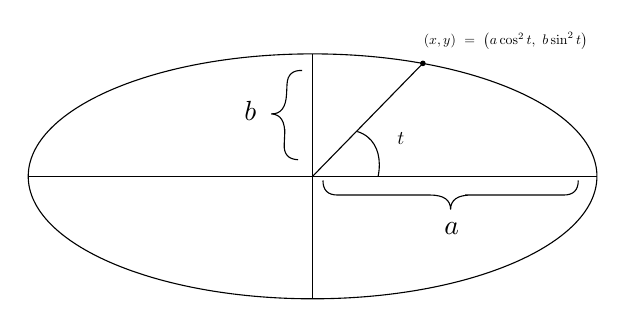
\begin{tikzpicture}[x=0.75pt,y=0.75pt,yscale=-1,xscale=1]
%uncomment if require: \path (0,300); %set diagram left start at 0, and has height of 300

%Shape: Ellipse [id:dp1559950964552308] 
\draw   (100,180) .. controls (100,147.42) and (161.34,121) .. (237,121) .. controls (312.66,121) and (374,147.42) .. (374,180) .. controls (374,212.58) and (312.66,239) .. (237,239) .. controls (161.34,239) and (100,212.58) .. (100,180) -- cycle ;
%Straight Lines [id:da3716259356733107] 
\draw    (100,180) -- (374,180) ;


%Straight Lines [id:da9880464900454329] 
\draw    (237,121) -- (237,239) ;


%Shape: Brace [id:dp3973633345998604] 
\draw   (242,182) .. controls (242,186.67) and (244.33,189) .. (249,189) -- (293.5,189) .. controls (300.17,189) and (303.5,191.33) .. (303.5,196) .. controls (303.5,191.33) and (306.83,189) .. (313.5,189)(310.5,189) -- (358,189) .. controls (362.67,189) and (365,186.67) .. (365,182) ;
%Shape: Brace [id:dp94498526835576] 
\draw   (232,129) .. controls (227.34,128.79) and (224.9,131.01) .. (224.68,135.67) -- (224.47,140.23) .. controls (224.16,146.89) and (221.68,150.11) .. (217.01,149.9) .. controls (221.68,150.11) and (223.85,153.55) .. (223.54,160.21)(223.68,157.21) -- (223.33,164.68) .. controls (223.12,169.35) and (225.34,171.79) .. (230,172) ;
%Shape: Arc [id:dp3154280429415799] 
\draw  [draw opacity=0] (258.54,158.43) .. controls (260.37,158.96) and (262.06,159.82) .. (263.54,161.03) .. controls (268.5,165.07) and (270.12,172.1) .. (268.62,179.79) -- (244.51,184.38) -- cycle ; \draw   (258.54,158.43) .. controls (260.37,158.96) and (262.06,159.82) .. (263.54,161.03) .. controls (268.5,165.07) and (270.12,172.1) .. (268.62,179.79) ;
%Shape: Circle [id:dp8908034615999807] 
\draw  [fill={rgb, 255:red, 0; green, 0; blue, 0 }  ,fill opacity=1 ] (289.08,125.57) .. controls (289.08,124.98) and (289.56,124.51) .. (290.14,124.51) .. controls (290.73,124.51) and (291.21,124.98) .. (291.21,125.57) .. controls (291.21,126.16) and (290.73,126.64) .. (290.14,126.64) .. controls (289.56,126.64) and (289.08,126.16) .. (289.08,125.57) -- cycle ;
%Straight Lines [id:da6323920079482996] 
\draw    (290.14,125.57) -- (237,180) ;



% Text Node
\draw (304,205) node   {$a$};
% Text Node
\draw (207,148.33) node   {$b$};
% Text Node
\draw (330,114.67) node [scale=0.5]  {$( x,y) \ =\ \left( a\cos^{2} t,\ b\sin^{2} t\right)$};
% Text Node
\draw (279.6,162) node [scale=0.7]  {$t$};


\end{tikzpicture}

    \fautor
    \label{fig:ellipse_params}
\end{figure}

Let $c \in \R^2$ be the center of an ellipse with shape parameters $(a,b) \in \R^2_{>0}$. Then $\gamma : [0, 2\pi] \mapsto \R^2$ defines a curve which maps every angle onto a point on the ellipse and it is defined as follows

    \begin{equation}\label{eq:parametric_ellipse}
    \gamma(t) = \left\{
    \begin{array}{l}
    x(t)= a\cos{t} + c_x\\
    y(t)=b\sin{t} + c_y
    \end{array}
    \right.
    \end{equation}

No equivalent disk-circle wording exists for ellipses, this could be a source of ambiguity in the text, that is why a note for the reader was judged to be necessary. Throughout this work an ellipse will represent the set of points that satisfy \autoref{def:ellipse}. In some places, though, with prior clarification, we will denote as an ellipse, the set of points that are covered by the ellipse itself. For example, when we define $\Pp \cap E$ as the set of points in $\Pp$ that are covered by $E$, we are implicitly calling $E$ the set of points that are covered by the ellipse itself as it is defined by \autoref{def:ellipse}.

\chapter{Maximal Covering by Disks}
\label{chapter:pmclp}
In this chapter, the classical version of PMCLP using disks will be defined and a version of the method will be proposed with the intention of later being used to solve the axis-parallel ellipses version of PMCLP. Throughout the course of this work, the maximal covering by disks problem is going to be referred to as $MCD(\Pp,m)$, where $\Pp$ is a set of points and $m$ is the number of unit disks.

\section{One disk, $MCD(\Pp,1)$}


Two exact methods for the $MCD(\Pp, 1)$ have been found in the literature. A $\bigO(n^2)$ algorithm is proposed by \cite{chazelle:1986} which improved the previously $\bigO(n^2\log{n})$ one proposed by \cite{drezner}.
As it has been mentioned, $MCD(\Pp,1)$ is a 3SUM-HARD problem, which means that it is as hard as the 3SUM problem (the problem of finding $3$ real numbers that sum to $0$, given $n$ real numbers). Initially the lower bound of the 3SUM problem was conjectured to be $\Omega(n^2)$, matching the best algorithm for $MCD(\Pp,1)$, which meant that no better time-complexity could be achieved. Since then, however, better algorithms for 3SUM have been developed with a $\bigO(\frac{n^2}{poly(n)})$ run time complexity \cite{3SUM-kopelowitz:2014}.

The $m=1$ version is treated here before the general case because it will be shown that, using the algorithm here proposed for $MCD(\Pp, 1)$, an optimal solution can be obtained for the $MCD(\Pp, m)$ as well as for the axis-parallel ellipse version of the problem.

\subsection{Notation and definition of the problem}

Initially, the input of the problem defines a unit disk with its center point undefined, a solution for the problem will then choose a point to be the center of the unit disk. In other words, a solution places the disk somewhere in the plane.
We refer to the unit disk with undefined center as $D$. If it is placed at a center $q \in \R^2$, we call it $D(q)$.

\begin{definicao}
    Let $\Pp=\{p_1,\dots,p_n\}$ be a set of $n$ points in $\R^2$ and $w(p)>0, p \in \Pp$, the weight of every point in $\Pp$. We denote $w(A)$, with $A \subset \Pp$, as the sum of weights of every point in $A$. Finally, let $D$ be a unit disk, we define an optimal solution of $MCD(\Pp,1)$ as
    
    \begin{equation}\label{eq:max_one_disk}
        \max_q w(\Pp \cap D(q)).
    \end{equation}

\end{definicao}

Therefore, an optimal solution for an instance of $MCD(\Pp,1)$ will be a point in which a unit disk located at, covers points whose weights, when summed, is maximal. 

In \cite{drezner}, the main idea used to develop the $\bigO(n^2\log{n})$ algorithm is that, even though there are infinitely many points where the disk could be placed, only a few of them, a finite amount of $\bigO(n^2)$, needs to be considered for the method to find an optimal one.
The algorithm, for every point, sorts the other points with respect to the angle they form with the first one. After that, the first point is placed on the border of the disk and, going through the sorted list, the algorithm inserts and removes points from the disk coverage. Also, when inserting and removing a point from the coverage, it only checks the disk centers that make the entering/leaving point to be on the border. Because the algorithm only checks the centers that make the disk have two points on its border, the number of centers it goes through is bounded by the number of pairs of points, which is $\binom{n}{2} = \bigO(n^2)$.

In \cite{chazelle:1986} and \cite{cabello:2006}, on the other hand, instead of working directly with $MCD(P,1)$, an equivalent problem called Maximum Weight Clique was introduced. The algorithm that we later describe in this work also uses this equivalence. That is why it has been taken to be fundamental to introduce the Maximum Weight Clique Problem and discuss the equivalence.




\section{Maximum Weight Clique Problem}

Let $\Pp=\{p_1,\dots,p_n\}$, with $p_i \in \R^2$, be a set of points, $\D=\{D_1,\dots,D_n\}$ a set of unit disks, such that $D_i$ is centered at $p_i$, $i=1,\dots,n$, with every disk having a weight $w_i > 0$, $i=1,\dots,n$. A clique, in this context, is a non-empty intersection area of a subset of disks. Note that this is different than the clique problem on a intersection graph (a graph where the vertices are the disks and an edge exists if there is an intersection between two disks). As shown in \autoref{fig:three_disks_no_intersection}, three disks could have non-empty pairwise intersection (which qualifies them as a clique), but the intersection of all the three together is empty. That is why the clique problem for unit disks is also referred to as the Maximum Geometric Clique Problem when the condition of common intersection exists and as the Maximum Graphical Clique Problem when there is only the pairwise intersection condition \cite{inplace:2014}. The graphical version of the problem was studied by \cite{graphical-clique}, where a $\bigO(n^{4.5})$ algorithm was proposed. Also, in \cite{inplace:2014}, a $\bigO(n^2\log{n})$ time in-place algorithm\footnote{An in-place algorithm is an algorithm that needs $\bigO(1)$ extra space.} for arbitrary radii disks was proposed. In \cite{chazelle:1986}, the method for the Maximum Geometric Weight Clique Problem consists on building a planar graph on which the vertices were the $\bigO(n^2)$ pairwise intersection of the circumferences and the edges were the arcs of the circumferences connecting the intersections. With the graph constructed, a traversal is done to obtain the answer, thus the time complexity of $\bigO(n^2)$.

\begin{figure}[H]
\centering

    \caption{Three disks that have non-empty pairwise intersection among them, but no common intersection.}
    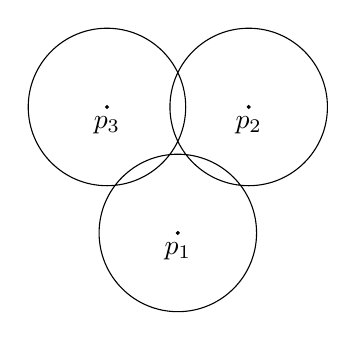
\begin{tikzpicture}[scale=1]
    %\draw [help lines] (-5,-3) grid (5,3);
    \draw (0,0) circle (1cm) (0.9,1.6) circle (1cm) (-0.9,1.6) circle (1cm);

    %a^2-b^2=c^2 -> c^2=25-9=16 -> c=4
    
    \draw[fill] (0.9,1.6) circle [radius=.5pt];
	\draw[fill] (0,0) circle [radius=.5pt];
    \draw[fill] (-0.9,1.6) circle [radius=.5pt];
    
    \node[below] at (0,0) {$p_1$};
    \node[below] at (0.9, 1.6) {$p_2$};
    \node[below] at (-0.9, 1.6) {$p_3$};
    
    %\draw [-] (-5,0) -- (5,0);
     %\draw [-] (0,-3) -- (0,3);
     %\draw [|-|] (0.001,-0.1) -- (4.999,-0.1);
    \end{tikzpicture}
    \label{fig:three_disks_no_intersection}
    \fautor
\end{figure}


A solution for the Maximum Weight Clique is a set of points $Q$, such that the sum of weights of all disks that cover it is maximized. Even though there could be a use for the whole set $Q$, as this problem is used as a tool to solve another problem, only finding a point from the Maximum Weight Clique is enough. This will become clear when the equivalence is stated. With everything in hands, we can define the Maximum Weight Clique Problem as follows.

\begin{definicao}\label{def:max_weight_clique}
    Let $\D$ be a set of unit disks and $\Pp$ be a set of points as defined before. An optimal solution for the Maximum Weight Clique Problem is given by 
    
    \begin{equation}
        \max_q \sum_{D_k \cap q \neq \emptyset} w_k.
    \end{equation}

\end{definicao}



As it has been proposed, with the equivalence of the two problems, an optimal solution of the Maximum Weight Clique Problem is also an optimal solution of the $MCD(\Pp,1)$, which means that a disk centered at $q$, defined in \autoref{def:max_weight_clique}, will have a maximal weight covering of the set $\Pp$.

Given an instance of $MCD(\Pp,1)$, the equivalent Maximum Weight Clique Problem is obtained by defining set $\D$ to contain the disks centered at $\Pp$ and setting the weight of every disk to be the weight of its corresponding point in $\Pp$. A disk $D_i$ will represent the area where a disk can be placed in order to cover $p_i$. This means that a intersection between some disks is an area where a disk could be placed to cover the corresponding points.

In \autoref{fig:three_disks_no_intersection}, it can be seen that there is no point where a disk could be placed such that it would cover $p_1, p_2$ and $p_3$, nonetheless, in any of the pairwise intersections, a disk could be placed to cover the two corresponding points.

Formally, in the Maximum Weight Clique Problem, if a point $q$ lies inside $\bigcap_{k \in I} D_k$, with $I \subset \{1,\dots,n\}$, then a disk centered at $q$ will cover the points $p_k$, with $k\in I$ in the $MCD(P,1)$ problem. Conversely, the same applies for a disk placed at $q$ that covers points $p_k$, with $k \in I$ in the one disk maximal covering problem. It means that $q$ will lie inside region $\bigcap_{k \in I} D_k$.

\subsection{An algorithm for the Maximum Weight Clique Problem}

The algorithm described here is based on the one in \cite{drezner}, also with some ideas from \cite{inplace:2014} and \cite{cabello:2006}. It has a run time complexity of $\bigO(n^2\log{n})$ and uses $\bigO(n)$ of extra space. It is worth noting, however, that a $\bigO((n+K)\log{n})$ run time, with $K$ being the number of intersections, can be obtained by using the algorithm in \cite{bentley:1979} to find all the intersections among the $n$ circumferences.

Without loss of generality, the weights will be ignored, and the method will be described for the Maximum Clique Problem, assuming that every disk has unit weight. Also, it will be assumed that no pair of disks are placed at the same center.

Let $\D$ be a set of $n$ unit disks, a non-empty intersection area of a subset of disks is convex and bounded by the arcs of the disks that are intersecting \cite{inplace:2014}.
With this observation, in order to find an optimal solution, it is sufficient to check, for every disk $D$, every intersection area that is bounded by its arc.

\begin{definicao}\label{def:inter_arc}
    Let $D_i$ and $D_j$ be two unit disks that intersect (at least at one point). Also let $(\theta_1, \theta_2) \in [0,2\pi]^2$ be the two angles that the circumferences induced by $D_i$ and $D_j$ intersect, with the condition that $(\theta_1,\theta_2)$ defines an arc (counter-clockwise order) of $D_i$ that is the border of $D_i \cap D_j$. If $D_i$ is tangent to $D_j$, then $\theta_1=\theta_2$. Then, define $\Gamma_+(i,j) = \theta_1$ and $\Gamma_-(i,j) = \theta_2$, also we refer to them as opening and closing intersection angles respectively.
\end{definicao}

\begin{figure}[H]
\centering

    \caption{Three disks and their intersection points.}
    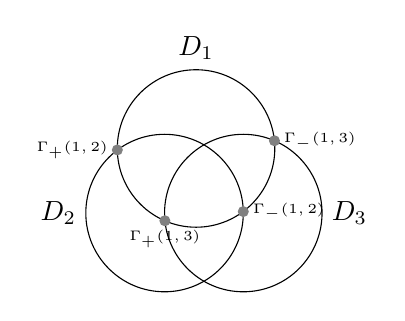
\begin{tikzpicture}
%\draw [help lines] (-5,-3) grid (5,3);

\draw[name path = c1] (0,0) circle (1cm);
\draw[name path = c3] (0.6,-0.82) circle (1cm);
\draw[name path = c2] (-0.4,-0.82) circle (1cm);

\node[above] at (0, 1) {$D_1$};
\node[left] at (-1.4, -0.82) {$D_2$};
\node[right] at (1.6, -0.82) {$D_3$};

\path [name intersections={of=c1 and c3}] ;
\foreach \i in {1,...,2}
\fill [color=gray] (intersection-\i) circle (2pt) ;

\node[right] at (intersection-1) {\tiny $\Gamma_-(1,3)$};
\node[left, below] at (intersection-2) {\tiny $\Gamma_+(1,3)$};

\path [name intersections={of=c1 and c2}] ;
\foreach \i in {1,...,2}
\fill [color=gray] (intersection-\i) circle (2pt) ;

\node[left] at (intersection-1) {\tiny $\Gamma_+(1,2)$};
\node[below,right] at (intersection-2) {\tiny $\Gamma_-(1,2)$};

%\draw [-] (-5,0) -- (5,0);
%\draw [-] (0,-3) -- (0,3);
%\draw [|-|] (0.001,-0.1) -- (4.999,-0.1);
\end{tikzpicture}
    \fautor
    \label{fig:3disks_intersect}
\end{figure}

In \autoref{fig:3disks_intersect}, it is shown all the intersection points between $D_1$ with $D_2$ and $D_3$. Also, they are labeled according to \autoref{def:inter_arc}. Note that $\Gamma_+(1,3) > \Gamma_-(1,3)$ (the angles should be in the $[0,2\pi]$ interval).

With \autoref{def:inter_arc} in hand, we can establish the basis of the algorithm to find the maximum clique in which a disk $D_i$ participates: a traversal going through every point of intersection with $D_i$, in counter-clockwise order, keeping a set of active disks. When an opening intersection angle is reached, the corresponding disk is added to the active set; when a closing one is reached, the corresponding disk is removed from the active set.
This simple traversal, however, would not handle the special case with $\Gamma_+(i,j) > \Gamma_-(i,j)$ (see \autoref{fig:3disks_intersect}). If the traversal begins at the point with smallest angle, the algorithm would remove $D_3$ from the active disks without first adding it. If there was another disk starting before $\Gamma_-(1,3)$, the algorithm would not have both of them in the active set at the same time, and an optimal solution could end up not being found. This can be worked around repeating the traversal once without resetting the active disks set, that way, in the beginning of the second traversal, the active set would contain the disks that have $\Gamma_+(i,j) > \Gamma_-(i,j)$. This is shown in \autoref{fig:array_disks}, where the intersections list is duplicated, simulating the traversal repetition (note the indication to where the traversal starts as well as the positive and negative signs representing when a intersection with another disk opens and closes, respectively). It can be seen that without the repetition, the algorithm would find $2$ as the value of an optimal solution, which is wrong.

\begin{figure}[H]
    \centering
    
    \caption{The intersections list of a disk with three other disks.}
    \usetikzlibrary{matrix}



\tikzset{every picture/.style={line width=0.75pt}} %set default line width to 0.75pt        

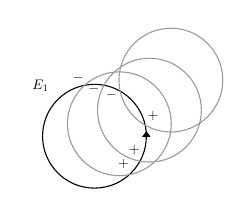
\begin{tikzpicture}[x=0.75pt,y=0.75pt,yscale=-1,xscale=1]
%uncomment if require: \path (0,95); %set diagram left start at 0, and has height of 95

%Shape: Circle [id:dp37777408295388804] 
\draw   (21,59.5) .. controls (21,45.69) and (32.19,34.5) .. (46,34.5) .. controls (59.81,34.5) and (71,45.69) .. (71,59.5) .. controls (71,73.31) and (59.81,84.5) .. (46,84.5) .. controls (32.19,84.5) and (21,73.31) .. (21,59.5) -- cycle ;
%Shape: Circle [id:dp4562198988843913] 
\draw  [color={rgb, 255:red, 155; green, 155; blue, 155 }  ,draw opacity=1 ] (47.5,46.94) .. controls (47.5,33.14) and (58.69,21.94) .. (72.5,21.94) .. controls (86.31,21.94) and (97.5,33.14) .. (97.5,46.94) .. controls (97.5,60.75) and (86.31,71.94) .. (72.5,71.94) .. controls (58.69,71.94) and (47.5,60.75) .. (47.5,46.94) -- cycle ;
%Shape: Circle [id:dp8913971633985722] 
\draw  [color={rgb, 255:red, 155; green, 155; blue, 155 }  ,draw opacity=1 ] (33,53.5) .. controls (33,39.69) and (44.19,28.5) .. (58,28.5) .. controls (71.81,28.5) and (83,39.69) .. (83,53.5) .. controls (83,67.31) and (71.81,78.5) .. (58,78.5) .. controls (44.19,78.5) and (33,67.31) .. (33,53.5) -- cycle ;
%Shape: Circle [id:dp05970043129919356] 
\draw  [color={rgb, 255:red, 155; green, 155; blue, 155 }  ,draw opacity=1 ] (57.81,32.47) .. controls (57.81,18.66) and (69,7.47) .. (82.81,7.47) .. controls (96.62,7.47) and (107.81,18.66) .. (107.81,32.47) .. controls (107.81,46.27) and (96.62,57.47) .. (82.81,57.47) .. controls (69,57.47) and (57.81,46.27) .. (57.81,32.47) -- cycle ;
%Straight Lines [id:da04725899028195979] 
%\draw[densely dotted]  (21,59.5) -- (71,59.5) ;


%Flowchart: Extract [id:dp5267407418119328] 
\draw  [fill={rgb, 255:red, 0; green, 0; blue, 0 }  ,fill opacity=1 ] (71,57.45) -- (72.52,59.55) -- (69.48,59.55) -- cycle ;

\draw (60,73) node [scale=0.5]  {$+$};
% Text Node
\draw (65.22,66) node [scale=0.5]  {$+$};
% Text Node
\draw (74.22,50) node [scale=0.5]  {$+$};
% Text Node
\draw (54.22,39.56) node [scale=0.5]  {$-$};
% Text Node
\draw (45.62,36.96) node [scale=0.5]  {$-$};
% Text Node
\draw (38.02,31.56) node [scale=0.5]  {$-$};


% Text Node
\draw (20,35) node [scale=0.5]  {$E_{1}$};
\end{tikzpicture}

\begin{tikzpicture}

\matrix [matrix of nodes,row sep=,row sep=0mm,
column 1/.style={nodes={rectangle,draw,minimum width=1.5em, minimum height=0.5em}},
column 2/.style={nodes={rectangle,draw,minimum width=1.5em, minimum height=0.5em}},
column 3/.style={nodes={rectangle,draw,minimum width=1.5em, minimum height=0.5em}},
column 4/.style={nodes={rectangle,draw,minimum width=1.5em, minimum height=0.5em}},
column 5/.style={nodes={rectangle,draw,minimum width=1.5em, minimum height=0.5em}},
column 6/.style={nodes={rectangle,draw,minimum width=1.5em, minimum height=0.5em}},
column 7/.style={nodes={rectangle,draw,minimum width=1.5em, color=gray, minimum height=0.5em}},
column 8/.style={nodes={rectangle,draw,minimum width=1.5em, color=gray, minimum height=0.5em}},
column 9/.style={nodes={rectangle,draw,minimum width=1.5em, color=gray, minimum height=0.5em}},
column 10/.style={nodes={rectangle,draw,minimum width=1.5em, color=gray, minimum height=0.5em}},
column 11/.style={nodes={rectangle,draw,minimum width=1.5em, color=gray, minimum height=0.5em}},
column 12/.style={nodes={rectangle,draw,minimum width=1.5em, color=gray, minimum height=0.5em}}
] (O)
{
$+$ & $-$ & $-$ & $-$ & $+$ & $+$ & $+$ & $-$ & $-$ & $-$ & $+$ & $+$\\
%$+$ & $-$ & $-$ & $-$ & $+$ & $+$\\
};

\node at (-4,-0.5) {$0$};
\node at (0,-0.5) {$2\pi$};
\end{tikzpicture}
    \fautor
    \label{fig:array_disks}
\end{figure}

\begin{algoritmo}
\caption{Algorithm for $MCD(\Pp, 1)$ with unit weights}\label{algoritmo:mcd_1}
\begin{algorithmic}[1]
\Require{A set of points $\Pp=\{p_1,\dots,p_n\}$.}
\Ensure{The maximum number of points that can be covered by a unit disk.}

\item[]

\Procedure{$MCD_1$}{$\Pp$}
\State $Q_{best} \gets \{\}$
\State $ans \gets$ center of $D_1$
\ForAll{$p_i \in \Pp$}
\State Let $D_i$ be the disk with center at $p_i$
\State Let $I_i$ be the set of disks that intersect with $D_i$
\State $A \gets \{\}$ \Comment{The multiset of intersection angles with $D_i$.}

\ForAll{$j \in I_i$}
\State $A \gets A \cup \{\Gamma_+(i,j) \cup \Gamma_-(i,j)\}$
\EndFor

%\State $A = \bigcup_{j \in I_i} \Gamma_+(i,j) \cup \Gamma_-(i,j)$
\State $Q \gets \{D_i\}$ \Comment{The set of active disks.}
\For{$cnt=1..2$} \Comment{Do it twice.}
\For{$a \in A$}\Comment{Assuming $A$ is sorted.}
\State Let $D_a$ be the disk that intersects $D_i$ at angle $a$. 
\If{$a$ is a starting angle}
\State $Q \gets Q \cup \{D_a\}$
\Else
\State $Q \gets Q \setminus \{D_a\}$
\EndIf
\If{$|Q_{best}| < |Q|$}
\State $Q_{best} \gets Q$
\State $ans \gets $ point corresponding to the intersection angle $a$
\EndIf
\EndFor
\EndFor
\EndFor

\State \Return $ans$
\EndProcedure
\end{algorithmic}
\end{algoritmo}

\begin{lema}\label{lema:disk}
\autoref{algoritmo:mcd_1} for solving the Maximum Clique Problem has a $\bigO((n+K)\log{n})$ run time complexity, where $K$ is the number of intersections of the $n$ disks.
\end{lema}

\begin{proof}
    Finding every intersection can be done in $\bigO((n+K)\log{n})$  by a plane sweep, the method is described in \cite{bentley:1979}. 
    Because the traversal is made in counter-clockwise order, the intersection points have to be sorted by their intersection angles, so an additional $\bigO(K\log{K})$ pre-processing is needed. All the other operations can be done in constant time. Therefore, the final algorithm complexity is $\bigO((n+K)\log{n})$.
\end{proof}

If a simpler implementation is desired, or the number of intersections is large, determining the set $I_i$ (the set of disks that intersect with $D_i$, defined in \autoref{algoritmo:mcd_1}) can be simply done in $\bigO(n^2)$, making the algorithm have a worst-case complexity of $\bigO(n^2\log{n})$.

\section{Multiple disks, $MCD(\Pp, m)$}


In \cite{cabello:2006}, a $\bigO(n^{2m-1}\log{n})$ algorithm for $MCD(\Pp, m)$ is developed as a sub-routine for its $(1-\epsilon)$-approximation algorithm. Firstly, they solve the sub-problem $MCD(\Pp, 2)$ in $\bigO(n^3\log{n})$. Then for the rest of the points that are not in that solution, it uses the algorithm developed in \cite{chazelle:1986} for the one-disk case, checking every possible solution for every one of the disks left.

Also, in \cite{zhou} an heuristic method for large-scale $MCD$ is proposed. It uses a probabilistic algorithm called mean-shift which is a gradient ascent method proven to converge to a local density maxima of any probability distribution. The mean-shift is utilized to find good candidates of centers for the unit disks, then the method backtracks to find the best assignment. The results showed that the greedy algorithm achieves an optimal coverage in some instances, but for some other ones it has a 15 percent worse coverage ratio.
 
It can be seen that in any solution of $MCD(\Pp, m)$, a disk placed at a point $q$ that covers at least one point $p \in \Pp$ has a correspondence to the Maximum Weight Clique Problem: the point $q$ is inside an intersection area of at least one disk and that area is bounded by some disk, which means it will be checked by \autoref{algoritmo:mcd_1} as a candidate to be an optimal solution. The number of points \autoref{algoritmo:mcd_1} goes through is $\bigO(n^2)$, then checking every possible center for every ellipse yields a $\bigO(n^{2m})$ run-time complexity.
This algorithm is described in \autoref{chapter:ellipses} for the ellipses case.

The choice of developing a different method for the problem, instead of using the one from \cite{cabello:2006}, is taken for the sake of simplicity, considering both algorithms achieve similar bounds.

\chapter{Maximal Covering by Ellipses}
\label{chapter:ellipses}
In this chapter, two versions of the planar maximal covering by ellipses problem will be introduced.
First, the axis-parallel variant will be defined and a method for it will be developed. Second, the version where there is no axis-parallel constraint and the ellipses can be freely rotated will be introduced.

\section{Axis-Parallel}
The maximal planar covering using axis-parallel ellipses was first introduced in \cite{canbolat} which proposed a mixed integer non-linear programming method for the problem. This first approach showed to be not that efficient as it could not find the optimal solution for some instances within a timeout defined by them. To obtain solutions, not necessarily optimal ones, for the instances which the exact method showed inefficiency, a heuristic technique called Simulated Annealing was used to develop another method. Comparisons were made which showed that the second approach was able to obtain good solutions, compared to the optimal ones found for some of the instances, within a good run-time.

The second work found in the literature was \cite{andreta} which developed a method that breaks the problem into smaller ones fixing the set of points an ellipse is going to cover. For each set of points fixed as the points an ellipse is going to cover, a small optimization problem is solved to find out if there is a location where the ellipse can be placed, so to cover the set of fixed points. To enumerate the possible solutions and then find the optimal one, the method defined a data structure that stores every set of points an ellipse can cover. This method showed better results and was able to find the optimal solutions for the instances that the first method could not get as well as for new created instances.

\subsection{Notation and definition of the problem}

Axis-parallel ellipses are defined as the set of points that satisfy \autoref{equation:pellipse}. Therefore, all it takes to describe one is a pair of positive real numbers $(a,b) \in \R_{>0}^2$, also called the shape parameters, and a center point $q \in \R^2$. 

Firstly, the case with only one ellipse is considered, an instance of the problem is denoted as $MCE(\Pp, a, b)$ where $\Pp$ is a set of points and $(a,b) \in \R_{>0}^2$, is a pair of real numbers called the shape parameters of an ellipse. 
In the general case every point has weights, but without loss of generality (later explained), this detail will be ignored and the weights are assumed to be unitary.
The notation used here is similar to the one introduced on \autoref{chapter:pmclp}, the ellipse with an undefined center is referred to as $E$. To denote the ellipse with center set to be at point $q$, $E(q)$ is used. Also, the set of points covered by $E(q)$ is denoted by $E(q) \cap \Pp$, which indirectly defines $E(q)$ to be the set of points that satisfy \autoref{equation:cover_pellipse}, in other words $E(q)$ is the coverage region defined by the ellipse with shape parameters $(a,b)$, located at center $q$. Hence, the problem can be defined as follows

\begin{definicao}
Let $MCE(\Pp, a, b)$ be an instance of the maximal covering by one ellipse, with $E$ being an ellipse with shape parameters $(a,b) \in \R_{>0}^2$, an optimal solution of $MCE(\Pp, a, b)$ is given by

\begin{equation}
    \max_q |\Pp \cap E(q)|
\end{equation}
\end{definicao}

\subsection{One Disk algorithm adaptation}

The adaptation of \autoref{algoritmo:mcd_1} is obtained by just replacing the function that finds the intersection points between two disks by a function that finds the intersection points between two ellipses.
It can be seen in \autoref{fig:3ellipses_intersect} that the intersection points and their correspondents $\Gamma_-(i,j)$ and $\Gamma_+(i,j)$ functions behave the same way as in the disks case.

The intersection of two ellipses as well as determining $\Gamma_-(i,j)$ and $\Gamma_+(i,j)$ is described thoroughly in \autoref{chapter:ellipses_intersection}. 


\begin{figure}[H]
\centering

    \caption{Three ellipses and their intersection points}
    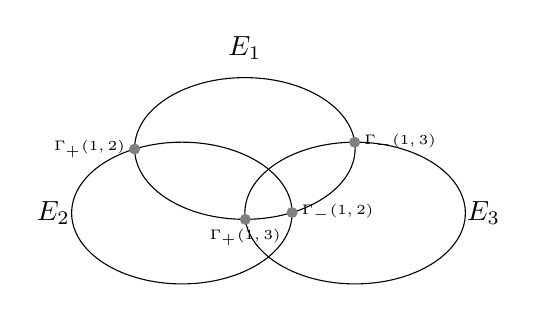
\begin{tikzpicture}
%\draw [help lines] (-5,-3) grid (5,3);

\draw[name path = c1] (0,0) ellipse (1.4cm and 0.9cm);
\draw[name path = c3] (1.4,-0.82) ellipse (1.4cm and 0.9cm);
\draw[name path = c2] (-0.8,-0.82) ellipse (1.4cm and 0.9cm);

\node[above] at (0, 1) {$E_1$};
\node[left] at (-2.1, -0.82) {$E_2$};
\node[right] at (2.7, -0.82) {$E_3$};

\path [name intersections={of=c1 and c3}] ;
\foreach \i in {1,...,2}
\fill [color=gray] (intersection-\i) circle (2pt) ;

\node[right] at (intersection-1) {\tiny $\Gamma_-(1,3)$};
\node[left, below] at (intersection-2) {\tiny $\Gamma_+(1,3)$};

\path [name intersections={of=c1 and c2}] ;
\foreach \i in {1,...,2}
\fill [color=gray] (intersection-\i) circle (2pt) ;

\node[left] at (intersection-1) {\tiny $\Gamma_+(1,2)$};
\node[below,right] at (intersection-2) {\tiny $\Gamma_-(1,2)$};

%\draw [-] (-5,0) -- (5,0);
%\draw [-] (0,-3) -- (0,3);
%\draw [|-|] (0.001,-0.1) -- (4.999,-0.1);
\end{tikzpicture}
    \fautor
    \label{fig:3ellipses_intersect}
\end{figure}

\subsection{Multiple ellipses}

The multiple ellipses case is handled using the same idea of the multiple disks case. The only difference is that an instance of the multiple ellipses may contain ellipses of different shapes, which does not happen for the disks case as every disk has the same radius. For this reason, a different pre-processing has to be done for every one of them.

An instance of the multiple ellipses case is denoted as $MCE(\Pp, \E)$, with $\Pp$ being a set of $n$ points and $\E = \{E_1, \dots, E_m\}$ being a set of $m$ ellipses, each one with shape parameters $(a_i, b_i) \in \R^2_{>0}, i = 1 \dots m$. Also, without loss of generality, the weight of every point is assumed to be unitary.

\begin{definicao}
Let $MCE(\Pp, \E)$ be an instance of the maximal covering by ellipses, an optimal solution is given by

\begin{equation}
    max_{q_1, \dots, q_m}{\left|\bigcup_{i=1}^{m} \Pp \cap E_i(q_i)\right|}
\end{equation}
\end{definicao}

The \autoref{algoritmo:mce} describes the adapted version of the maximal disk covering algorithm for the ellipses case. The $MCE_1$ procedure returns every possible set of points that an ellipse with shape parameters $(a,b)$ can cover. With that, the procedure $MCE$ does the backtracking process, assigning every possible cover to every ellipse.

As stated in \autoref{lema:disk}, $MCE_1$ runs in $\bigO(n^2\log{n})$. The number of sets of points an ellipse can cover, however, is $\bigO(n^2)$, note that the $\log{n}$ is part of the complexity due to sorting the set $A$. If $MCE_1$ is called only in a pre-process phase storing its return for every ellipse, a $\bigO(n^{2m})$ run-time complexity can be achieved. 

Also, it can be seen that the unitary weights assumption can be easily removed through replacing the way the answer is updated: 
the weights of the covered points should be added to the answer instead of the number of covered points, this could be done by keeping an extra variable along with every possible set of points an ellipse can cover that is returned by $MCE_1$.

It is worth noting that some easy improvements, which do not change the algorithm's overall complexity, can be made in the implementation. For example, if an ellipse covers two sets of points $X$ and $Y$, with $X \subset Y$, then set $X$ can be ignored by the algorithm because of the positive weights constraint. Also, if two ellipses have their centers with euclidean distance greater than their semi-major parameter, they for sure do not intersect. Depending on the input, this observation can make the algorithm not go through the whole list of ellipses every time it needs to determine the ellipses pairwise intersections.



\begin{algoritmo}[b]
\caption{Algorithm for $MCE(\Pp, \E)$ with unit weights}\label{algoritmo:mce}
\begin{algorithmic}[1]
\Procedure{$MCE_1$}{$\Pp, a, b$}\Comment{Returns every possible coverage.}
\State $Q \gets \{\}$

\ForAll{$p_i \in \Pp$}
\State Let $E_i$ be the ellipse with center at $p_i$ and parameters $(a,b)$

\State Let $I_i$ be the set of ellipses that intersect with $E_i$

\State $A = \bigcup_{j \in I_i} \Gamma_+(i,j) \cup \Gamma_-(i,j)$

\State $Q \gets Q \cup \{p_i\}$ 
\State $Cov \gets \{p_i\}$ \Comment{The set of active disks}

\For{$cnt=1..2$} \Comment{Do it twice}
\For{$a \in A$}\Comment{Assuming $A$ is sorted}
\State Let $p_a$ be the point represented by the ellipse that intersects $E_i$ at angle $a$. 
\If{$a$ is a starting angle}
\State $Cov \gets Cov \cup \{p_a\}$
\Else
\State $Cov \gets Cov \setminus \{p_a\}$
\EndIf
\State $Q \gets Q \cup Cov$
\EndFor
\EndFor
\EndFor

\State \Return $Q$
\EndProcedure

\Procedure{$MCE$}{$\Pp, \E, j=1$}\Comment{Returns an optimal solution of $MCE(\Pp, \E)$, $j$ is a backtracking parameter that says that $j$-th ellipse should be processed by this call.}
\If{$j = m+1$}
\State \Return $0$
\EndIf

\State $ans \gets 0$
\For{$E \in \E$}
\State Let $(a,b)$ be the shape parameters of $E$
\State $Q \gets MCE_1(\Pp, a, b)$
\For{$Cov \in Q$}
\State $ans \gets \max\{ans, |Cov| + MCE(\Pp \setminus Cov, \E, j+1 \}$ \Comment{Calls the procedure for the next ellipse}
\EndFor
\EndFor

\State \Return $ans$
\EndProcedure
\end{algorithmic}
\end{algoritmo}
 

\chapter{Future Work}
\label{chapter:future_work}
To take advantage of the great amount of work found in the literature,
 we decided to first introduce the planar maximal covering by disks problem, develop a method for it, and just then adapt it for the ellipses case. It turned out that because of the similarities between the two problems, adapting was possible and actually very simple. This made the method developed by us have a very different approach than the ones in \cite{andreta} and \cite{canbolat}. The next step is to implement it and compare the results that \cite{andreta} obtained.
 
As of future work, we intend to study the $(1-\epsilon)$-approximation method for the planar covering with disks in \cite{cabello:2006} and develop an adapted version of the algorithm for ellipses with the same time complexity of $\bigO(n\log{n})$.

Also, the version of the problem where every ellipse can be freely rotated is set as a primary goal for this master's research. In \cite{andreta}, the deterministic method developed by them could not obtain solutions for moderate-to-large instances within reasonable time. Because of that, a stochastic global optimization method was proposed, it performed well and was able to obtain an optimal solution for small cases. The goal we have in mind for the future is to develop an exact method that takes into consideration the algorithm we developed for the axis-parallel version of the problem and compare the results.

Finally, as a secondary goal, we want to develop a probabilistic approximation algorithm based on \cite{aronov:2008} which proposed a Monte Carlo approximation for the problem of finding the deepest point in a arrangement of regions. The method runs in $\bigO(n\epsilon^2\log{n})$ and can be applied to solve the case with one ellipse. The case with more than one ellipse is left as a challenge for us for the next steps of our research.



%\chapter{Orientações gerais}
%\label{chapter:orientacoes-gerais}
%
\section{Codificação dos arquivos: UTF8}

A codificação de todos os arquivos do pacote \abnTeX, incluindo a classe \textit{icmc}, é \texttt{UTF8}. É necessário que
você utilize a mesma codificação nos documentos que escrever, inclusive nos
arquivos de base bibliográficas |.bib|.



\section{Inclusão de outros arquivos}\label{sec-include}

É uma boa prática dividir o seu documento em diversos arquivos, e não
apenas escrever tudo em um único. Para tanto, esse recurso foi utilizado neste
documento, além de estarem organizados em um diretório separado do arquivo principal. Para incluir diferentes arquivos em um arquivo principal,
de modo que cada arquivo incluído fique em uma página diferente, utilize o
comando:

\begin{verbatim}
   \include{tex/documento-a-ser-incluido}    % sem a extensão .tex
\end{verbatim}

Para incluir documentos sem quebra de páginas, utilize:

\begin{verbatim}
   \input{tex/documento-a-ser-incluido}      % sem a extensão .tex
\end{verbatim}



\section{Remissões internas}

Ao nomear a \autoref{tab:lista_produtos} e a \autoref{fig:logomarca_usp}, apresentamos um exemplo de remissão interna, que também pode ser feita quando indicamos o \autoref{chapter:corpos-flutuantes}, que tem o nome \emph{\nameref{chapter:corpos-flutuantes}}. O número do capítulo indicado é \ref{chapter:corpos-flutuantes}, que se inicia à \autopageref{chapter:corpos-flutuantes}\footnote{O número da página de uma remissão pode ser obtida também assim:
\pageref{chapter:corpos-flutuantes}.}.

O código usado para produzir o texto desta seção é:

\begin{verbatim}
Ao nomear a \autoref{tab:lista_produtos} e a \autoref{fig:logomarca_usp}, 
apresentamos um exemplo de remissão interna, que também pode ser feita 
quando indicamos o \autoref{chapter:corpos-flutuantes}, que tem o nome 
\emph{\nameref{chapter:corpos-flutuantes}}. O número do capítulo indicado 
é \ref{chapter:corpos-flutuantes}, que se inicia à 
\autopageref{chapter:corpos-flutuantes}
\footnote{O número da página de uma remissão pode ser obtida também assim: 
\pageref{chapter:corpos-flutuantes}.}.
\end{verbatim}

\section{Diferentes idiomas e hifenizações}
\label{sec-hifenizacao}

Para usar hifenizações de diferentes idiomas, inclua nas opções do documento o nome dos idiomas que o seu texto contém. Por exemplo (para melhor visualização, as opções foram quebras em diferentes linhas):

\begin{verbatim}
    \documentclass[
        qualificacao,
        mestrado
        pos-defesa,
        english,
        french,
        spanish,
        brazil
    ]{icmc}
\end{verbatim}

Os idiomas português-brasileiro (\texttt{brazil}) e inglês (\texttt{english}) são incluídos automaticamente pela classe \textsf{icmc}. Caso deseje utilizar outros idiomas no corpo do documento, como em citações em francês, você deve usar o preâmbulo como abaixo:

\begin{verbatim}
    \documentclass[
        doutorado,
        pre-defesa,
        french
    ]{icmc}
\end{verbatim}

A lista completa de idiomas suportados, bem como outras opções de hifenização, estão disponíveis em \citeonline[p.~5-6]{babel}.


\section{Comandos auxiliares úteis}

A classe \textit{icmc} contém alguns comandos auxiliares definidos com o objetivo de tornar o processo de escrita mais eficiente. Os principais comandos são apresentados a seguir:

\begin{description}
    
    \item[\comando{aspas\{CONTENT\}}] Comando utilizado para inserir um texto entre aspas.
    \item[\comando{autoref\{LABEL\}}] Comando utilizado para fazer referência a um elemento do texto. O parâmetro \texttt{LABEL} utilizado refere-se ao código definido por meio do comando \comando{label\{\}}.
    \item[\comando{fadaptada[CONTENT]\{REF\}}] Comando utilizado nos ambientes de \texttt{Figura}, \texttt{Tabela}, entre outros, para definir a origem da fonte do dado apresentado que foi adaptado de alguma referência. Os parâmetros utilizados são: \texttt{REF} que é o índice da referência no arquivo bibtex, e; \texttt{CONTENT} que é a localização exata do dado na referência (Ex.: p~30). O parâmetro \texttt{CONTENT} é opcional.
    \item[\comando{fautor}] Comando utilizado nos ambientes de \texttt{Figura}, \texttt{Tabela}, \texttt{Quadro}, entre outros, que define o próprio autor como provedor da informação.
    \item[\comando{fdadospesquisa}] Comando utilizado nos ambientes de \texttt{Figura}, \texttt{Tabela}, \texttt{Quadro}, entre outros, que define que os dados originaram da própria pesquisa.
    \item[\comando{fdireta[CONTENT]\{REF\}}] Comando utilizado nos ambientes de \texttt{Figura}, \texttt{Tabela}, \texttt{Quadro}, entre outros, para definir a origem da fonte do dado apresentado que foi adaptado de alguma referência. Os parâmetros utilizados são: \texttt{REF} que é o índice da referência no arquivo bibtex, e; \texttt{CONTENT} que é a localização exata do dado na referência (Ex.: p~30). O parâmetro \texttt{CONTENT} é opcional.
    \item[\comando{newword\{WORD\}\{DESC\}}] Comando utilizado para inserir palavras no glossário de modo mais prático. Os parâmetros utilizados são: \texttt{WORD} que é a palavra que será descrita, e; \texttt{DESC} que é o significado da palavra.
    \item[\comando{rev\{CONTENT\}}] Comando utilizado para inserir notas de revisão dentro do texto, as quais aparecerão destacadas em vermelho. O parâmetro utilizado é \texttt{CONTENT} que contém o texto sobre a revisão.
    \item[\comando{sigla\{ABBR\}\{DESC\}}] Comando utilizado para inserir siglas e abreviaturas na Lista de siglas de modo mais prático. Os parâmetros utilizados são: \texttt{ABBR} que é a abreviatura ou sigla, e \texttt{DESC} sua descrição. Ao utilizar esse comando, a sigla \textbf{também} é inserida no texto do documento.
    \item[\comando{sigla*\{ABBR\}\{DESC\}}] Comando utilizado para inserir siglas e abreviaturas na Lista de Siglas de modo mais prático. Os parâmetros utilizados são: \texttt{ABBR} que é a abreviatura ou sigla, e \texttt{DESC} sua descrição. Ao utilizar esse comando, a sigla é inserida \textbf{apenas} na Lista de Siglas.
    \item[\comando{simbolo\{SYM\}\{DESC\}}] Comando utilizado para inserir símbolos na Lista de Símbolos de modo mais prático. Os parâmetros utilizados são: \texttt{SYM} que é o símbolo, e \texttt{DESC} sua descrição. 
    
\end{description}


\section{Consulte o manual da classe \textsf{abntex2}}

Consulte o manual da classe \textsf{abntex2} \cite{abntex2classe} para uma
referência completa das macros e ambientes disponíveis. 

Além disso, o manual possui informações adicionais sobre as normas ABNT
observadas pelo \abnTeX\ e considerações sobre eventuais requisitos específicos, como o caso da \citeonline[seção 5.2.2]{NBR14724:2011}, que
especifica o espaçamento entre os capítulos e o início do texto.



\section{Precisa de ajuda?}

Consulte a FAQ com perguntas frequentes e comuns no portal do \abnTeX:
\url{https://code.google.com/p/abntex2/wiki/FAQ}.

Inscreva-se no grupo de usuários \LaTeX:
\url{http://groups.google.com/group/latex-br}, tire suas dúvidas e ajude
outros usuários.

Participe também do grupo de desenvolvedores do \abnTeX:
\url{http://groups.google.com/group/abntex2} e faça sua contribuição à
ferramenta.


\section{Você pode ajudar?}

Sua contribuição é muito importante! Você pode ajudar na divulgação,
desenvolvimento, aprimoramento e de várias outras formas. Veja como contribuir com a classe \textit{icmc} em
\url{https://github.com/lordantonelli/thesis-model-icmc} e faça sua contribuição.


%\chapter{Configuração dos elementos pré-textuais}
%\label{chapter:config-pre-textual}
%A configuração de diversas opções e principalmente dos elementos pré-textuais é realizada com comandos específicos inseridos antes do comando \comando{begin\{document\}}. As informações do documento são configuradas através dos comandos:

\begin{description}

 \item[\comando{tituloPT\{T\}}] Título do trabalho em português (substitua T pelo título do trabalho em português);
 
 \item[\comando{tituloEN\{T\}}] Título do trabalho em inglês (substitua T pelo título do trabalho em inglês);

 \item[\comando{autor[REF]\{N\}}] Nome do autor do trabalho (onde REF é como o nome do autor é referenciado e N é o nome do autor);
 
  \item[\comando{genero\{GEN\}}] Gênero do autor. Substitua GEN pela sigla do gênero correspondente (M = Masculino ou F = Feminino);

 \item[\comando{orientador\{T\}\{O\}}] Nome do professor orientador do trabalho. Caso seja uma orientadora pode ser usado o comando \comando{orientador[Orientadora]\{T\}\{O\}} (sendo que T é a titulação do professor e O é o nome do orientador);

 \item[\comando{coorientador\{T\}\{C\}}] Nome do professor coorientador do trabalho. Caso seja uma coorientadora pode ser usado um comando análogo a definição de orientadora  empregando o comando \comando{coorientador[Coorientadora]\{T\}\{C\}}(sendo que T é a titulação do professor e C é o nome do orientador);

 
 \item[\comando{curso\{SPPG\}}] Dados do programa de Pós-Graduação, onde SPPG é a sigla do programa de pós-graduação. Exemplo: \comando{curso\{CCMC\}}. Os seguintes programas de Pós-Graduação estão disponíveis e configurados neste \textit{template}:
    \begin{itemize}
        \item \textbf{CCMC} -- Programa de Pós-Graduação em Ciências de Computação e Matemática Computacional
        \item \textbf{MAT} -- Programa de Pós-Graduação em Matemática
        \item \textbf{PIPGES} -- Programa Interinstitucional de Pós-Graduação em Estatística
        \item \textbf{PROFMAT} -- Programa de Pós-Graduação em Mestrado Profissional em Matemática em Rede Nacional
        \item \textbf{MECAI} -- Programa de Pós-Graduação em Mestrado Profissional em Matemática, Estatística e Computação Aplicadas à Indústria
    \end{itemize}
 
 \item[\comando{data\{dia\}\{mês\}\{ano\}}] Configuração da data do depósito do documento;
 
 \item[\comando{idioma\{LANG\}}] Definição do idioma principal que o documento será escrito. As opções disponíveis são: \textbf{PT} (para escrita em português) e \textbf{EN} (para escrita em inglês), que devem obrigatoriamente serem informadas em letras maiúsculas.

 \item[\comando{textoresumo\{TR\}\{PC\}}] Texto do resumo (TR) e palavras-chave (PC) do documento sendo separadas por vírgula. Se o idioma do resumo for diferente do declarado no documento, pode ser usado o comando \comando{textoresumo[L]\{TR\}\{PC\}} (sendo que L é a linguagem do resumo);
 
 \item[\comando{incluifichacatalografica\{ARQ\}}] Inclusão da ficha catalográfica do documento gerada diretamente no site da biblioteca \url{http://www.icmc.usp.br/Portal/Sistemas/Biblioteca/ficha.php}, em que ARQ é o nome do arquivo PDF, incluindo o caminho do diretório se necessário.

 
\end{description}

As opções seguintes correspondem também as configurações dos elementos pré-textuais, porém seu uso é opcional: 

\begin{description}

 \item[\comando{textodedicatoria\{TD\}}] Texto referente a dedicatória do trabalho (TD). Caso o texto esteja em um arquivo separado (recomendado para que o projeto fique modularizado e os documentos mais limpo), deve utilizar o comando \comando{textodedicatoria*\{ARQ\}}, em que ARQ é o nome do arquivo, incluindo o caminho do diretório se necessário;

 \item[\comando{textoagradecimentos\{TA\}}] Texto referente aos agradecimentos do trabalho (TA). Caso o texto esteja em um arquivo separado (recomendado para que o projeto fique modularizado e os documentos mais limpo), deve utilizar o comando \comando{textoagradecimentos*\{ARQ\}}, em que ARQ é o nome do arquivo, incluindo o caminho do diretório se necessário;

 \item[\comando{incluilistadefiguras}] Comando para inclusão da lista de figuras. Deve-se utilizar este comando somente quando o ambiente \textbf{figure} for utilizado no documento;
 
 \item[\comando{incluilistadetabelas}] Comando para inclusão da lista de tabelas. Deve-se utilizar este comando somente quando o ambiente \textbf{table} for utilizado no documento;
  
 \item[\comando{incluilistadequadros}] Comando para inclusão da lista de quadros. Deve-se utilizar este comando somente quando o ambiente \textbf{quadro} for utilizado no documento;
   
 \item[\comando{incluilistadealgoritmos}] Comando para inclusão da lista de algoritmos. Deve-se utilizar este comando somente quando o ambiente \textbf{algoritmo} for utilizado no documento;
    
 \item[\comando{incluilistadecodigos}] Comando para inclusão da lista de figuras. Deve-se utilizar este comando somente quando o ambiente \textbf{codigo} for utilizado no documento;
 
 \item[\comando{incluilistadesiglas}] Comando para inclusão da lista de siglas e abreviaturas. Deve-se utilizar este comando somente quando existirem siglas e abreviaturas no documento, com a utilização do comando \comando{sigla\{S\}\{DS\}} ou \comando{sigla*\{S\}\{DS\}};

 \item[\comando{incluilistadesimbolos}] Comando para inclusão da lista de símbolos. Deve-se utilizar este comando somente quando existirem símbolos no documento, com a utilização do comando \comando{simbolo\{S\}\{DS\}}.
 
\end{description}

%\chapter{Corpos flutuantes}
%\label{chapter:corpos-flutuantes}
%
Corpos flutuantes são elementos não textuais, como figuras e tabelas, que complementam as informações do texto. Neste capítulo são expostos breves exemplos dos corpos flutuantes disponíveis na classe \textit{icmc}.

Na \autoref{secao:figuras} é mostrado como inserir figuras, a \autoref{secao:tabelas_e_quadros} explica como incluir tabelas e quadros, a \autoref{secao:algoritmos_e_codigos} demostra como trabalhar com algoritmos e códigos-fonte e a \autoref{secao:outros-ambientes} explica como definir outros ambientes para serem utilizados, como para gráficos e diagramas.

\section{Figuras}
\label{secao:figuras}

A inserção de figuras é realizada normalmente através do comando \comando{begin\{figure\}}. Na \autoref{fig:logomarca_usp} é exibida a logomarca da USP com o pacote \textit{graphicx}. Já a \autoref{figura:exemplo_grafo} mostra um exemplo de grafo com o pacote \textit{xy}. Na \autoref{fig:animals} pode ser visto um exemplo de utilização de subfiguras. De acordo com as normas ABNT a lista de figuras é um elemento opcional do documento, para incluí-la é preciso inserir o comando \comando{incluidelistafiguras} antes do início do documento.

Observe que, segundo a \citeonline[seções 4.2.1.10 e 5.8]{NBR14724:2011}, as
ilustrações devem sempre ter numeração contínua e única em todo o documento. Além disso, deve ser incorporado ao corpo flutuante do tipo figura, além da legenda, a fonte de onde esta foi extraída. Se a figura foi confeccionada pelo próprio autor, deve se colocar "Elaborada pelo autor".

\begin{citacao}
Qualquer que seja o tipo de ilustração, sua identificação aparece na parte
superior, precedida da palavra designativa (desenho, esquema, fluxograma,
fotografia, gráfico, mapa, organograma, planta, quadro, retrato, figura,
imagem, entre outros), seguida de seu número de ordem de ocorrência no texto,
em algarismos arábicos, travessão e do respectivo título. Após a ilustração, na
parte inferior, indicar a fonte consultada (elemento obrigatório, mesmo que
seja produção do próprio autor), legenda, notas e outras informações
necessárias à sua compreensão (se houver). A ilustração deve ser citada no
texto e inserida o mais próximo possível do trecho a que se
refere. \cite[seções 5.8]{NBR14724:2011}
\end{citacao}

\begin{figure}[htb]
 \caption{Logomarca da USP}
 \label{fig:logomarca_usp}
 \centering
 
\includegraphics[scale=0.23]{usp-logo.pdf}
 \fdireta{usp:logo}
\end{figure}


\begin{figure}[htb]
\caption{Exemplo de grafo}
\label{figura:exemplo_grafo}
\centering
\begin{scriptsize}
$$
\xymatrix@R20pt@C10pt{
 & & & & vr \ar[dlll] \ar[dl] \ar[d] \ar[dr] \ar[drr] \ar[drrr] & & & \\
 & (a_3, b_2, c_1) \ar[d]^{\varphi_2} \ar[dl]_{\varphi_1} & & (a_3, b_2, c_2) \ar[d]^{\varphi_2} \ar[dl]_{\varphi_1} & (a_1, b_1, c_1) & (a_1, b_1, c_2) & (a_1, b_2, c_1) & (a_1, b_2, c_2) \\
 (a_2, b_2, c_1) \ar[dr]_{\varphi_3} & (a_3, b_1, c_1) \ar[d]^{\varphi_1} & (a_2, b_2, c_2) \ar[dr]_{\varphi_3} & (a_3, b_1, c_2) \ar[d]^{\varphi_1} & & & & \\
& (a_2, b_1, c_1)  & & (a_2, b_1, c_2) & & & & \\
}
$$
\end{scriptsize}
\fautor
\end{figure}

\begin{figure}[htb] 
    \centering 
    \caption{Figuras de animaisPictures of animals}\label{fig:animals} 
    \begin{subfigure}[b]{0.317\textwidth} 
        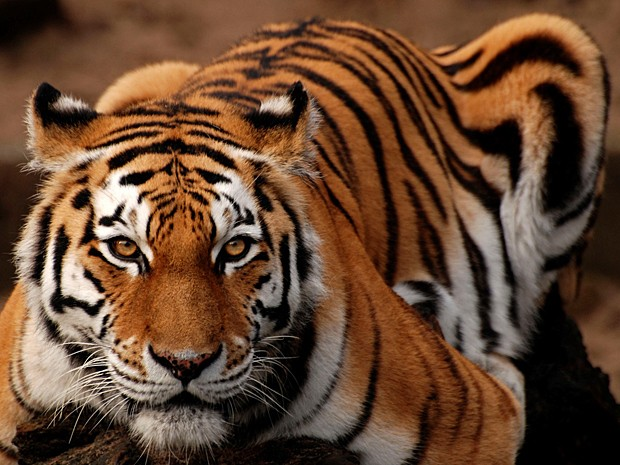
\includegraphics[width=\textwidth]{tigre.jpg} 
        \caption{Tigre} 
        \label{fig:tigre} 
    \end{subfigure} ~ %add desired spacing between images, e. g. ~, \quad, \qquad, \hfill etc. %(or a blank line to force the subfigure onto a new line) 
    \begin{subfigure}[b]{0.317\textwidth} 
        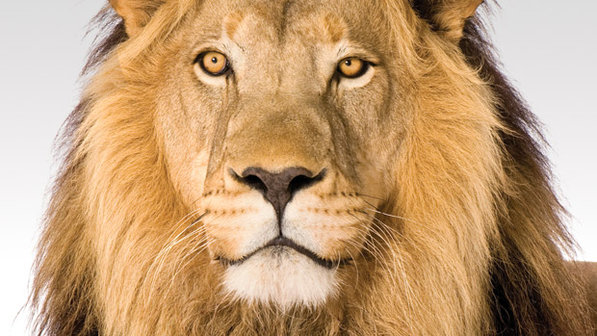
\includegraphics[width=\textwidth]{leao.jpg} 
        \caption{Leão} \label{fig:leao} 
    \end{subfigure} ~ %add desired spacing between images, e. g. ~, \quad, \qquad, \hfill etc. %(or a blank line to force the subfigure onto a new line) 
    \begin{subfigure}[b]{0.317\textwidth} 
        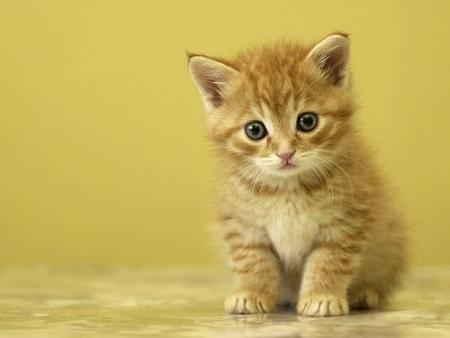
\includegraphics[width=\textwidth]{gato.jpg} 
        \caption{Gato} \label{fig:gato} 
    \end{subfigure}
    \fautor
\end{figure}

A classe \textit{icmc} traz algum comando que auxiliam na inserção da legenda, para utilizá-los basta substituir o \comando{fonte\{\}} por um dos seguintes comando conforme necessário:

\begin{description}

 \item[\comando{fautor}] Insere o texto \aspas{Elaborada pelo autor} como fonte da figura;

 \item[\comando{fadaptada[INF]\{REF\}}] Insere um texto informando que a figura foi adaptada de alguma referência bibliográfica (REF). INF refere-se ao local específico de onde a imagem foi extraída, como por exemplo o número da página. Além disso, INF é um parâmetro opcional e pode receber qualquer cadeia de texto;

 \item[\comando{fdireta[INF]\{REF\}}] Insere um texto informando que a figura próvem diretamente de alguma referência bibliográfica (REF). INF refere-se ao local específico de onde a imagem foi extraída, como por exemplo o número da página. Além disso, INF é um parâmetro opcional e pode receber qualquer cadeia de texto;
 
 \item[\comando{fdadospesquisa}] Insere o texto \aspas{Dados da pesquisa.} como fonte da figura;
 
\end{description}




\section{Tabelas e Quadros}
\label{secao:tabelas_e_quadros}

A inserção de tabelas e quadros é feita de forma semelhante a inserção de figuras, porém são utilizados os ambientes \textit{table} e \textit{quadro}. A principal diferença entre tabelas e quadros, de acordo com \citeonline{NBR14724:2011}, é que as tabelas são destinadas para informações numéricas e os quadros são mais adequados para informações textuais. Em geral, as tabelas devem estar padronizadas conforme o padrão do \citeonline{ibge1993} requerido pelas normas da ABNT para documentos técnicos e acadêmicos.

Como exemplos foram inseridas a \autoref{tab:lista_produtos} que exibe uma de lista de produtos (construída em \LaTeX) e a Tabela \autoref{tabela:populacao_america_sul} que mostra a população dos países da América do Sul (construída segundo o padrão do IBGE). Foi inserido também o \autoref{quadro:editores_texto_livres} com alguns editores que podem ser usados para se trabalhar com \LaTeX para demonstrar a inserção de quadros.

 A lista de tabelas também é um elemento opcional que pode ser incluída com o comando \comando{incluidelistatabelas} antes do início do documento. O mesmo acontece com a lista de quadros que pode ser incluída com o comando \comando{incluidelistaquadros}.

\begin{table}[htb]
\centering
\caption{Lista de produtos}
\label{tab:lista_produtos}
\begin{tabularx}{\textwidth}{X|l|r|r|r} \hline
Produto      & Unidade & Preço (R\$) & Quantidade & Total (R\$) \\ \hline
Arroz        & Kg      & 2,00        & 550        & 1.100,00    \\
Óleo de Soja & L       & 2,50        & 500        & 750,00      \\
Açucar       & Kg      & 3,00        & 100        & 300,00      \\ \hline
\end{tabularx}
\fdadospesquisa
\end{table}

\begin{table}[htb]
\IBGEtab{%
  \caption{População dos países da América do Sul} \label{tabela:populacao_america_sul}
}{%
\begin{tabular}{r|p{6.3cm}|r}        
\toprule
Código  & País            & População   \\ \midrule \midrule
1       & Brasil          & ~~~~~~191.480.630 \\ \midrule 
2       & Argentina       &  39.934.100 \\ \midrule 
3       & Colômbia        &  46.741.100 \\ \midrule 
4       & Paraguai        &   9.694.200 \\ \midrule 
5       & Uruguai         &   3.350.500 \\ \midrule 
6       & Peru            &  28.221.500 \\ \midrule 
7       & Equador         &  13.481.200 \\ \midrule 
8       & Bolívia         &   9.694.200 \\ \midrule 
9       & Venezuela       &  28.121.700 \\ \midrule 
10      & Chile           &  16.803.000 \\ \bottomrule
\end{tabular}
}{%
  \fdireta{wikipedia:2011:america_sul}%
  \nota{Esta é uma nota, que diz que os dados são baseados na
  regressão linear.}%
  \nota[Anotações]{Uma anotação adicional, que pode ser seguida de várias
  outras, porém são opcionais.}%
  }
\end{table}

\begin{quadro}[htb]
\caption{Editores de Texto Livres}
\label{quadro:editores_texto_livres}
\centering
\begin{tabular}{|l|l|r|}        \hline
Editor     & Multiplataforma & Específico para Latex \\ \hline
Kwriter    & Sim             & Não                   \\
Texmaker   & Sim             & Sim                   \\
Kile       & Sim             & Sim                   \\
Geany      & Sim             & Não                   \\ \hline
\end{tabular}
\end{quadro}

\section{Algoritmos e Códigos}
\label{secao:algoritmos_e_codigos}

Além dos corpos flutuantes convencionais para inserir figuras (\comando{begin\{figure\}}) e tabelas (\comando{begin\{table\}}), a classe \textit{icmc} possui mais dois tipos de corpos flutuantes um para algoritmos (\comando{begin\{algoritmo\}}) e outro para códigos-fonte (\comando{begin\{codigo\}}). A utilização de um ou de outro fica a critério do usuário. Como exemplo temos o \autoref{algoritmo:euclidalgoritmo:mdc1} que calcula o máximo divisor comum entre dois números e os Códigos-fonte \ref{codigo:notas_alunos} e \ref{codigo:metodo_leitura} que são uma consulta na \sigla{SQL}{\textit{Structured Query Language}} e uma sobrotina em \textit{Java}.


%\begin{algoritmo}
%\caption{Algoritmo para cálculo de máximo divisor comum MDC($n_1$,$n_2$)}
%\label{algoritmo:mdc1}
%
% \KwIn{Dois números inteiros ($n_1, n_2$)}
% \If(\tcp*[f]{Garante que o maior número seja $n_1$}){$n_2 > n_1$}
%   {troca valores de $n_1$ e $n_2$}
% \Repeat{$r > 0$}{
%    $r \leftarrow$ resto da divisão de $n_1$ por $n_2$
%    $n_1 \leftarrow n_2$
%    $n_2 \leftarrow r$
% }
% \Return $n_1$
%\end{algoritmo}

\begin{codigo}[caption = {Consulta SQL}, label={codigo:notas_alunos},language=SQL, breaklines=true]
SELECT a.nome_aluno AS aluno,
       d.nome_disciplina AS disciplina,
       m.nota AS nota
FROM aluno AS a,
     disciplina AS d,
     matriculado AS m
WHERE a.id_aluno = m.id_aluno
  AND d.id_disciplina = m.id_disciplina
ORDER BY a.nome_aluno, d.nome_disciplina;
\end{codigo}

\begin{codigo}[caption={Subrotina para obter uma entrada do usuário}, label={codigo:metodo_leitura}, language=Java, breaklines=true]
public static String Leitura(){
    BufferedReader reader = new BufferedReader(new InputStreamReader(System.in));
    try {
        return reader.readLine(); // Lê uma linha pelo teclado
    } catch (IOException e) {
        e.printStackTrace();
        return "";
    }
}
\end{codigo}

\begin{algoritmo}
\caption{Algoritmo de Euclides}\label{algoritmo:euclidalgoritmo:mdc1}
\begin{algorithmic}[1]
\Procedure{Euclid}{$a,b$}\Comment{O maior divisor comum de \textit{a} e \textit{b}}
\State $r\gets a\bmod b$
\While{$r\not=0$}\Comment{Tem-se a resposta se \textit{r} é 0}
\State $a\gets b$
\State $b\gets r$
\State $r\gets a\bmod b$
\EndWhile\label{euclidendwhile}
\State \Return $b$\Comment{O maior divisor comum é \textit{b}}
\EndProcedure
\end{algorithmic}
\end{algoritmo}

Existem diversos outros pacotes disponíveis para escrever algoritmos e códigos. Nos exemplos anteriormente foram utilizados o pacote \textit{algorithmicxalgorithm} para definição do ambiente algoritmo e \textit{listings} para a definição do ambiente de código-fonte. O pacote \textit{algorithmicxalgorithm} é usado para escrever algoritmos em alto nível \cite{janos:2005:algpseudocode}. Já o pacote \textit{listings} serve para escrever os códigos em diversas linguagens de programação \cite{moses:2006:listings}.

Caso sejam utilizados os ambientes de algoritmos e código podem ser incluídos os comandos \comando{incluidelistaalgoritmos} e \comando{incluidelistacodigos} antes do \comando{begin\{document\}} para que a lista de algoritmos e a lista de código sejam criadas.


\section{Ambientes Matemáticos}

A classe \textit{icmc} provê os seguintes ambientes matemáticos:
\begin{itemize}
 \item Teoremas (\comando{begin\{teorema\}[\ ]} ... \comando{begin\{teorema\}});
 \item Proposição (\comando{begin\{proposicao\}[\ ]} ... \comando{begin\{proposicao\}});
 \item Lema (\comando{begin\{lema\}[\ ]} ... \comando{begin\{lema\}});
 \item Corolário (\comando{begin\{corolario\}[\ ]} ... \comando{begin\{corolario\}});
 \item Exemplo (\comando{begin\{exemplo\}[\ ]} ... \comando{begin\{exemplo\}});
 \item Observação (\comando{begin\{observacao\}[\ ]} ... \comando{begin\{observacao\}});
 \item Definição (\comando{begin\{definicao\}[\ ]} ... \comando{begin\{definicao\}});
 \item demonstracao (\comando{begin\{demonstracao\}[\ ]} ... \comando{begin\{demonstracao\}}).
\end{itemize}

Abaixo temos um exemplo de proposição com sua demonstração:
\begin{proposicao}
 Sejam $a$ e $b$ reais, tais que $0<a<b$. Então $a^2<b^2$.
\end{proposicao}
\begin{demonstracao}
 Pela hipótese concluímos que $(b+a)>0$ e $(b-a)>0$.

Como $b^2-a^2=(b+a)(b-a)$ concluímos que $b^2-a^2>0$, ou seja, $a^2<b^2$.
\end{demonstracao}

Neste documento tratamos brevemente apenas dos ambientes mencionados anteriormente. Contudo, para escrever expressões matemáticas complexas é preciso estudar uma documentação mais específica como em \citeonline{cassagojr:1997:amslatex}.

Alguns dos ambientes matemáticos da classe \textit{icmc} podem ser usados também para outras finalidades como exemplos e definições.


\section{Definição de outros ambientes}
\label{secao:outros-ambientes}

O classe \textit{icmc} permite a criação de outros ambientes, além dos citados nas seções anteriores, caso seja necessário. Isso é possível graças a extensão da classe \textit{abntex}. O \autoref{codigo:novo-ambiente} deve ser inserido antes do início do documento para criação de um ambiente para gráficos. Para definição de outros ambientes, basta seguir o modelo.


\begin{codigo}[caption={Definição do ambiente \textbf{grafico}}, label={codigo:novo-ambiente}, language=Tex, breaklines=true]
\makeatletter

% Novo list of (listings) para GRÁFICOS --------------------------
\newcommand{\graficoname}{Gráfico}
\newcommand{\graficorefname}{Gráfico}
\newcommand{\listofgraficosname}{Lista de gráficos}

\addto\captionsenglish{% ingles
    %% adjusts names from abnTeX2
    \newcommand{\graficoname}{Graph}
    \newcommand{\graficorefname}{Graph}
    \newcommand{\listofgraficosname}{List of graphs}
}

\newalgoritmo:euclid{grafico}{htbp}{logr}[chapter]
\floatname{grafico}{\graficoname}
\restylefloat{grafico}
\newfloat[chapter]{grafico}{logr}{\graficoname}
\newlistof{listofgraficos}{logr}{\listgraficoname}
\newlistentry{grafico}{logr}{0}

% configurações para atender às regras da ABNT
\renewcommand{\thegrafico}{\thechapter.\@arabic\c@grafico}
\setfloatadjustment{grafico}{\centering}
\renewcommand{\cftgraficoname}{\graficoname\space}
\renewcommand*{\cftgraficoaftersnum}{\hfill\textendash\hfill}
% -----------------------------------------------------------

\makeatother
\end{codigo}

A utilização do novo ambiente no texto segue conforme o \autoref{codigo:usar-novo-ambiente}.

\begin{codigo}[caption={Como usar o ambiente \textbf{grafico}}, label={codigo:usar-novo-ambiente}, language=Tex, breaklines=true]
\begin{grafico}[htb]
\caption{Caption do gráfico}
\label{gra:modelo}
Este é o conteúdo do gráfico.
\end{grafico}
\end{codigo}

Comandos como \comando{autoref\{gra:modelo\}} funcionam normalmente.

Para imprimir a "Lista de gráficos" no documento, insira o \autoref{codigo:lista-novo-ambiente} na classe \textit{icmc}, de modo que ele seja impresso após a "Lista de ilustrações". O código deve ser inserido após a linha 1244.


\begin{codigo}[caption={Código para inserir lista de gráficos}, label={codigo:lista-novo-ambiente}, language=Tex, breaklines=true]
% ---
% inserir lista de gráficos
% ---
\pdfbookmark[0]{\listofgraficosname}{logr}
\listofgraficos*
\cleardoublepage
% ---
\end{codigo}

%\chapter{Listas}
%\label{chapter:listas}
%\section{Abreviaturas e Siglas}

A classe \textit{icmc} implementa a criação da lista de abreviaturas e siglas com o pacote \textit{nomencl}. A inserção de abreviaturas e siglas na lista é realizada com o comando \comando{sigla\{A\}\{B\}} que também insere o conteúdo da sigla no local do documento onde a mesma foi definida. Os parâmetros utilizados são: \textit{A} que é a sigla e \textit{B} que é o nome por extenso. Caso deseja-se inserir a sigla apenas na lista, pode-se utilizar o comando \comando{sigla*\{A\}\{B\}}.

Para se gerar a lista de siglas na parte pre-textual do documento é preciso incluir o comando \comando{incluidelistasiglas} antes do início do documento. Além disto, a compilação do documento deve conter o comando \textit{makeindex} após duas compilações com o \textit{pdflatex}. Por exemplo, supondo que o documento principal tenha o nome de \textit{thesis}, podemos usar a seguinte sequência de comandos:

\begin{verbatim}
pdflatex thesis.tex
pdflatex thesis.tex
makeindex thesis.nlo -s nomencl.ist -o thesis.nls
pdflatex thesis.tex
\end{verbatim}

No \autoref{chapter:ferramentas-uteis} serão apresentadas algumas ferramentas que podem facilitar o processo de compilação do documento. Em especial, o ShareLaTeX não necessita de um processo de compilação especial para gerar a lista de abreviaturas e siglas.


\section{Símbolos}

A definição de símbolos é semelhante a definição de siglas, porém deve ser usado o comando \comando{simbolo\{S\}\{DS\}}, onde \textit{S} é o símbolo e \textit{DS} é a descrição do símbolo. Como exemplo definimos os símbolos $\mathbb{X}$\simbolo{\mathbb{X}}{Variável X} e $\mathsf{I\!R}$\simbolo{\mathsf{I\!R}}{Conjunto dos números reais}. Para incluir a lista de símbolos, basta usar o comando \comando{incluidelistasimbolos} antes do início do documento.


%\chapter{Ferramentas úteis}
%\label{chapter:ferramentas-uteis}
%Existem diversas ferramentas para se trabalhar com \LaTeX. Três ferramentas que merecem destaque são o editor \textit{Texmaker} (\autoref{fig:texmaker}), o ShareLaTeX (\autoref{fig:sharelatex}) e o gerenciador de referências \textit{JabRef} (\autoref{fig:jabref}). Todas as ferramentas são livres e multiplataforma. 

\begin{figure}[htb]
\caption{Tela do Texmaker}
 \label{fig:texmaker}
 \centering
 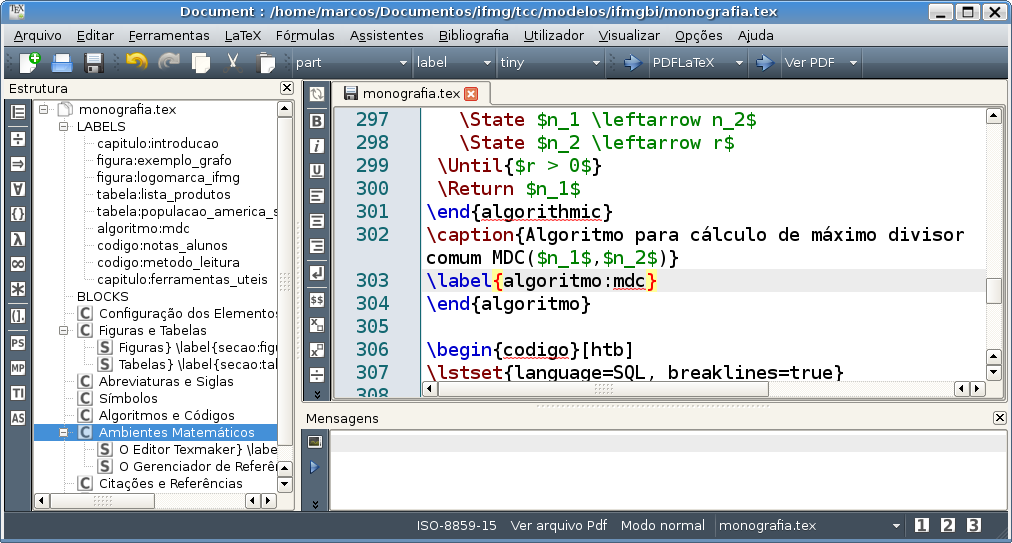
\includegraphics[width=\textwidth]{texmaker.png}
 \fautor
\end{figure}

\begin{figure}[htb]
\caption{Site do ShareLaTeX}
 \label{fig:sharelatex}
 \centering
 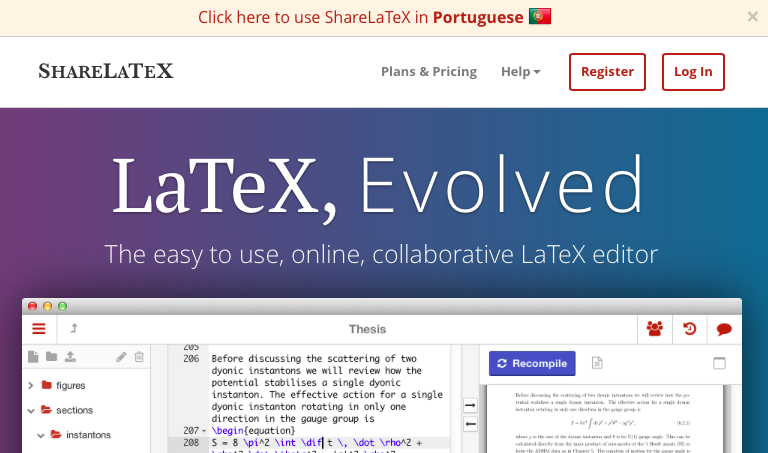
\includegraphics[scale=0.5]{sharelatex.png}
 \fautor
\end{figure}

\begin{figure}[htb]
 \caption{Tela do JabRef}
 \label{fig:jabref}
 \centering
 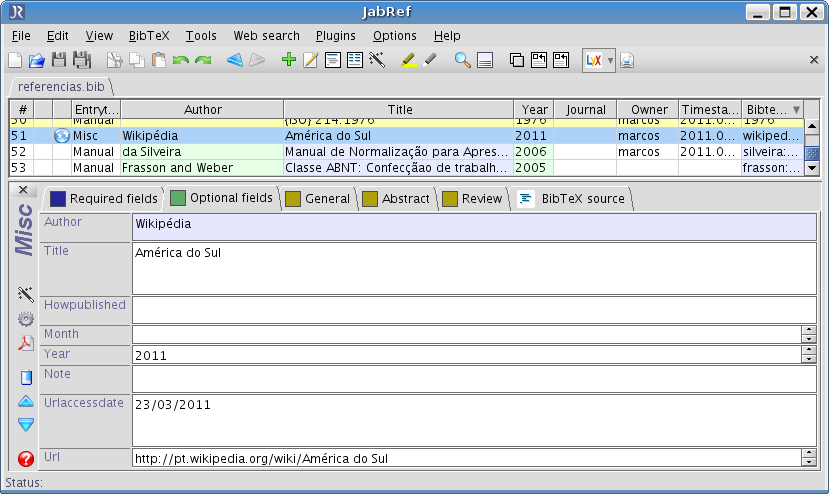
\includegraphics[scale=0.45]{jabref.png}
\fautor
\end{figure}

O Texmaker pode ser obtido em \url{www.xm1math.net/texmaker} e o JabRef pode ser obtido em \url{jabref.sourceforge.ne}. É importante ressaltar que o Texmaker é apenas um editor, para compilar os documentos é necessário um ambiente \LaTeX instalado. Os ambientes Latex mais populares são o Texlive (\url{www.tug.org/texlive}) e o MiKTex (\url{miktex.org}). 

As estrutura de referências do bibtex utilizadas nesse \textit{template} contém alguns parâmetros adicionais que o modelo geral não tem, conforme pode ser consultado em \citeonline{abntex2cite-alf}. Desta forma, recomenda-se fortemente o uso do gerenciador de referências JabRef, uma vez que é possível customizá-lo para atender estas exigências. O código de customização pode ser visto no \autoref{chapter:configuracao-jabref}.

O ShareLaTeX é uma ferramenta de edição de documento em \LaTeX de forma online e está disponível em \url{www.sharelatex.com}. A ferramenta permite o compartilhamento e edição simultânea do conteúdo. Além disso, pode-se consultar o histórico da edições realizadas no documento. A principal vantagem de utilizar o ShareLaTeX é não precisar instalar o compilador para LaTeX.

%\chapter{Citações e referências}
%\label{chapter:citacoes}
%

Em documentos acadêmicos podem existir as citações podem ser: \textbf{implícitas} quando as referências não fazem parte do texto ou \textbf{explícitas} quando o autor referente a citação é mencionado explicitamente na sentença. Nesse sentido, deve-se utilizar os comandos específicos para cada tipo de citação, ou seja, em citações explicitas deve-se usar o comando \comando{citeonline\{\}} e nas demais situações é usado o comando \comando{cite\{\}}. Alguns exemplos são apresentados no \autoref{qua:exemplo-citacao}.

\begin{quadro}[htb]
\caption{Exemplos de citações no documento}
\label{qua:exemplo-citacao}
\centering\small 
\begin{tabular}{|c|c|}        \hline
\textbf{Código em \LaTeX} & \textbf{Código Compilado}\\ \hline\hline
\begin{minipage}[t]{\VerbL}
\vspace{5pt}
\begin{verbatim}
A ironia será assim uma ... proposta
por \citeonline{10520:2000:4.1-1}.
\end{verbatim}
\vspace{5pt}
\end{minipage}
&
\begin{minipage}[t]{\LatL}
\vspace{5pt}
A ironia será assim uma ... proposta 
por \citeonline{10520:2000:4.1-1}.
\vspace{5pt}
\end{minipage}\\\hline

\begin{minipage}[t]{\VerbL}
\vspace{5pt}
\begin{verbatim}
\citeonline[p.~146]{10520:2000:4.2-2}
dizem que ... 
\end{verbatim}
\vspace{5pt}
\end{minipage}
&
\begin{minipage}[t]{\LatL}
\vspace{5pt}
\citeonline[p.~146]{10520:2000:4.2-2} dizem que {...}
\vspace{5pt}
\end{minipage}\\ \hline

\begin{minipage}[t]{\VerbL}
\vspace{5pt}
\begin{verbatim}
``Apesar das ... da filosofia''
\cite[p.~293]{10520:2000:4.1-2}.
\end{verbatim}
\vspace{5pt}
\end{minipage}
&
\begin{minipage}[t]{\LatL}
\vspace{5pt}
``Apesar das {...} da filosofia'' \cite[p.~293]{10520:2000:4.1-2}.
\vspace{5pt}
\end{minipage} \\ \hline

\begin{minipage}[t]{\VerbL}
\vspace{5pt}
\begin{verbatim}
Depois, ...  que prefiro
\cite{10520:2000:4.1-3}.
\end{verbatim}
\vspace{5pt}
\end{minipage}
&
\begin{minipage}[t]{\LatL}
\vspace{5pt}
Depois, {...} que prefiro \cite{10520:2000:4.1-3}.
\vspace{5pt}
\end{minipage}\\ \hline

\end{tabular}
\end{quadro}


Para especificar a página, seção ou capítulo consultado na referência é preciso acrescentá-lo entre colchetes com os comandos \comando{cite[página]\{\}} ou \comando{citeonline[página]\{\}}. O texto colocado entre colchetes aparecerá logo após o ano. Maiores informações sobre os comandos utilizados para citação posem ser consultados no manual de referência da abnTeX2, incluindo o uso de \textbf{apud} \cite{abntex2cite-alf}.


\section{Citações Indiretas}

As citações indiretas são caracterizadas como uma espécie de paráfrase das ideias de um determinado autor, ou seja, o pesquisador, por meio de suas próprias palavras, interpreta o discurso de outrem, contudo, mantendo o mesmo sentido. Outro aspecto que deve ser considerado é a necessidade de o autor (ou os autores) e o ano em que a obra foi publicada serem mencionados. 

Nas citações indiretas há duas formatações possíveis dependendo de como ocorre a citação no texto. Quando o autor é mencionado explicitamente utiliza-se o comando \comando{citeonline\{\}}, caso contrário, deve utilizar o comando \comando{cite\{\}}. 



\section{Citações diretas}
\label{sec-citacao}


As citações diretas ocorrem quando o texto de uma referência é transcrito literalmente. As citações diretas curtas (até três linhas) são inseridas no texto entre aspas duplas. As aspas simples são utilizadas para indicar citação no interior da citação: \aspas{Nas citações, as chamadas pelo sobrenome do autor [...] incluído na sentença devem ser em letras maiúsculas e minúsculas e, quando estiverem entre parênteses, devem ser em letras maiúsculas} \cite[sec.~5]{NBR10520:2002}.

\begin{verbatim}
``Nas citações, as chamadas pelo sobrenome do autor [...] incluído na 
sentença devem ser em letras maiúsculas e minúsculas e, quando 
estiverem entre parênteses, devem ser em letras maiúsculas''
\cite[5]{NBR10520:2002}.
\end{verbatim}

Cabe ressaltar que em \LaTeX as aspas iniciais são diferentes das finais. Para tanto, pode-se utilizar o comando \comando{aspas\{CONTEUDO\}} para inserir um determinado conteúdo entre aspas.

As citações diretas longas (com mais de 3 linhas) podem ser inseridas por meio do ambiente \texttt{citacao}:

\begin{citacao}
As citações diretas, no texto, com mais de três linhas, devem ser
destacadas com recuo de 4 cm da margem esquerda, com letra menor que a do texto
utilizado e sem as aspas. No caso de documentos datilografados, deve-se
observar apenas o recuo \cite[5.3]{NBR10520:2002}.
\end{citacao}

Use o ambiente assim:

\begin{verbatim}
\begin{citacao}
As citações diretas, no texto, com mais de três linhas [...] deve-se 
observar apenas o recuo \cite[5.3]{NBR10520:2002}.
\end{citacao}
\end{verbatim}

O ambiente \texttt{citacao} pode receber como parâmetro opcional um nome de
idioma previamente carregado nas opções da classe (\autoref{sec-hifenizacao}). Nesse
caso, o texto da citação é automaticamente escrito em itálico e a hifenização é
ajustada para o idioma selecionado na opção do ambiente. Por exemplo:

\begin{verbatim}
\begin{citacao}[english]
Text in English language in italic with correct hyphenation.
\end{citacao}
\end{verbatim}

Tem como resultado:

\begin{citacao}[english]
Text in English language in italic with correct hyphenation.
\end{citacao}



% ---
% Finaliza a parte no bookmark do PDF, para que se inicie o bookmark na raiz
% ---
\bookmarksetup{startatroot}% 
% ---

% ----------------------------------------------------------
% ELEMENTOS PÓS-TEXTUAIS
% ----------------------------------------------------------
\postextual

% ----------------------------------------------------------
% Referências bibliográficas
% ----------------------------------------------------------
\bibliography{references}

% ---------------------------------------------------------------------
% GLOSSÁRIO
% ---------------------------------------------------------------------

% Arquivo que contém as definições que vão aparecer no glossário
\newword{WYSIWYG}{``What You See Is What You Get''  ou ``O que você vê é o que você obtém''.  Recurso tem por objetivo permitir que um documento, enquanto manipulado na tela, tenha a mesma aparência de sua utilização, usualmente sendo considerada final. Isso facilita para o desenvolvedor que pode trabalhar visualizando a aparência do documento sem precisar salvar em vários momentos e abrir em um \textit{software} separado de visualização}
\newword{Framework}{é uma abstração que une códigos comuns entre vários projetos de \textit{software} provendo uma funcionalidade genérica. \textit{Frameworks} são projetados com a intenção de facilitar o desenvolvimento de \textit{software}, habilitando designers e programadores a gastarem mais tempo determinando as exigências do \textit{software} do que com detalhes de baixo nível do sistema}

\newword{Template}{é um documento sem conteúdo, com apenas a apresentação visual (apenas cabeçalhos por exemplo) e instruções sobre onde e qual tipo de conteúdo deve entrar a cada parcela da apresentação}

\newword{Padrões de projeto}{ou \textit{Design Pattern}, descreve uma solução geral reutilizável para um problema recorrente no desenvolvimento de sistemas de \textit{software} orientados a objetos. Não é um código final, é uma descrição ou modelo de como resolver o problema do qual trata, que pode ser usada em muitas situações diferentes}

\newword{Web}{Sinônimo mais conhecido de \textit{World Wide Web} (WWW). É a interface gráfica da Internet que torna os serviços disponíveis totalmente transparentes para o usuário e ainda possibilita a manipulação multimídia da informação}

% Comando para incluir todas as definições do arquivo glossario.tex
%\glsaddall
% Impressão do glossário
%\printglossaries

% ----------------------------------------------------------
% Apêndices
% ----------------------------------------------------------

% ---
% Inicia os apêndices
% ---
\begin{apendicesenv}

    %\chapter{Documento básico usando a classe \textit{icmc}}
    %\label{chapter:documento-basico}
    %
\definecolor{gray}{rgb}{0.4,0.4,0.4}
\definecolor{darkblue}{rgb}{0.0,0.0,0.6}
\definecolor{cyan}{rgb}{0.0,0.6,0.6}
\definecolor{maroon}{rgb}{0.5,0,0}
\definecolor{darkgreen}{rgb}{0,0.5,0}


\lstdefinelanguage{myLatex}
{
    keywords={\titulo},
    alsoletter={-},
    sensitive=false,
    morecomment=[l]{\%},
    morecomment=[s]{/*}{*/},
    morestring=[b]",
    morestring=[b]',
    keywordstyle=\bfseries\color{blue},
    commentstyle=\itshape\color{darkgreen},
    morekeywords={documentclass, titulo, autor, data, orientador, coorientador, curso, textoresumo, incluifichacatalografica, textodedicatoria*, textoagradecimentos*, textoepigrafe*, incluilistadefiguras, incluilistadetabelas, incluilistadequadros, incluilistadealgoritmos, incluilistadecodigos, incluilistadesiglas, incluilistadesimbolos, textual, chapter, postextual, begin, bibliography, end}, 
alsoletter={*, \{, \}, \[, \]},
 morekeywords=[2]{\{, \}, \[, \]},
 keywordstyle=[2]\bfseries\color{blue},
 moredelim=[s][\color{maroon}]{\{}{\}},
    moredelim=[s][\itshape\color{maroon}]{\[}{\]},
}

%\lstdefinelanguage{TeX}
%{
%moredelim=*[s][\color{maroon}]{\{}{\}}
%otherkeywords={\{, \}, \[, \], \\}
%  morestring=[b]",
%  moredelim=[s][\bfseries\color{maroon}]{<}{\ },
%  moredelim=[s][\bfseries\color{maroon}]{</}{>},
%  moredelim=[l][\bfseries\color{maroon}]{/>},
%  moredelim=[l][\bfseries\color{maroon}]{>},
%  commentstyle=\color{darkgreen},
%  stringstyle=\color{blue},
%  identifierstyle=\color{red},
%  keywordstyle=\bfseries\color{maroon}
%moredelim=[l][\bfseries\color{maroon}]{>},
%commentstyle=\color{darkgreen},
%  stringstyle=\color{blue},
%  identifierstyle=\color{red}, moredelim=[l][\bfseries\color{maroon}]{\{},
%  keywordstyle=\bfseries\color{maroon}
%}

%\lstset{language={[LaTeX]TeX},
%texcsstyle=*\bfseries\color{blue},
%keywordstyle=\bfseries\color{blue},
%commentstyle=\color{darkgreen},
%morecomment=[s][\color{red}]{\{}{\}},
%otherkeywords={$, \{, \}, \[, \]}
%}

%\begin{codigo}[caption={Exemplo de um documento básico}, label={codigo:documento-basico}, language={[LaTeX]TeX},  breaklines=true,morekeywords={titulo, autor, data, orientador, coorientador, curso, textoresumo, incluifichacatalografica, textodedicatoria*, textoagradecimentos*, textoepigrafe*, incluilistadefiguras, incluilistadetabelas, incluilistadequadros, incluilistadealgoritmos, incluilistadecodigos, incluilistadesiglas, incluilistadesimbolos, {\backslash}textual, chapter, postextual}, alsoletter={{\backslash},*},morecomment=[s][\color{red}]{\{}{\}}]
\begin{codigo}[caption={Exemplo de um documento básico}, label={codigo:documento-basico}, language={myLatex},  breaklines=true]
% Documento utilizando a classe icmc
% Opções: 
%   Qualificação          = qualificacao 
%   Curso                 = doutorado/mestrado
%   Situação do trabalho  = pre-defesa/pos-defesa (exceto para qualificação)
%   Versão para impressão = impressao
\ documentclass[doutorado, pos-defesa]{packages/icmc}

% Título do trabalho em Português
\tituloPT{Título da Monografia}

% Título do trabalho em Inglês
\tituloEN{Título da Monografia}

% Nome do autor
\autor[Abreviação]{Nome completo do autor}

% Gênero do autor (M ou F)
\genero{M}

% Data do depósito
\data{18}{12}{2012}

% Nome do Orientador
\orientador[Orientador]{Titulação do orientador}{Nome completo do Orientador}

% Nome do Coorientador (caso não exista basta remover)
\coorientador[Coorientador]{Titulação do coorientador}{Nome completo do Coorientador}
% Se coorientadora troque Coorientador: por Coorientadora dentro do colchetes

% Sigla do programa de Pós-graduação (CCMC, MAT, PIPGES, PROFMAT, MECAI)
\curso{CCMC}
% O valor entre colchetes é opcional para este programa

% Idioma principal do texto (EN ou PT)
\idioma{PT}

% Resumo
\textoresumo[Idioma]{
Texto do resumo do trabalho.
}{Lista de palavras-chave separada por virgulas}

% ----------------------------------------------------------
% ELEMENTOS PRÉ-TEXTUAIS
% ----------------------------------------------------------

% Inserir a ficha catalográfica
\incluifichacatalografica{tex/ficha-catalografica.pdf}

% Incluí o texto da Dedicatória
\textodedicatoria*{tex/pre-textual/dedicatoria}

% Incluí o texto dos Agradecimentos
\textoagradecimentos*{tex/pre-textual/agradecimentos}

% Incluí o texto da Epígrafe
\textoepigrafe*{tex/pre-textual/epigrafe}

% Inclui a lista de figuras
\incluilistadefiguras

% Inclui a lista de tabelas
\incluilistadetabelas

% Inclui a lista de quadros
\incluilistadequadros

% Inclui a lista de algoritmos
\incluilistadealgoritmos

% Inclui a lista de códigos
\incluilistadecodigos

% Inclui a lista de siglas e abreviaturas
\incluilistadesiglas

% Inclui a lista de símbolos
\incluilistadesimbolos

% Início do documento
\begin{document}

% ----------------------------------------------------------
% ELEMENTOS TEXTUAIS
% ----------------------------------------------------------
\textual

\chapter{Introdução}

Capítulo de Introdução

\chapter{Desenvolvimento}

Capítulo de Desenvolvimento

\chapter{Conclusão}

Capítulo de conclusão

% ----------------------------------------------------------
% ELEMENTOS PÓS-TEXTUAIS
% ----------------------------------------------------------
\postextual

% Nome do arquivo com as referências bibliográficas
\bibliography{referencias}

\end{document}

\end{codigo}
    
    
    \chapter{Intersections of two ellipses}
    \label{chapter:ellipses_intersection}
    In this appendix the intersection of two ellipses with the same shape parameters $(a,b) \in \R^2_{>0}$ is described with more detail, as well as determining the functions $\Gamma_+(i,j)$ and $\Gamma_-(i,j)$ for two ellipses that intersect.

\section{Intersection}

Let $E_1$ and $E_2$ be two ellipses that the intersection will be determined here. Without loss of generality, let us assume that $E_1$ is at the origin and $E_2$ is located at the center $(h,k) \in \R^2$. Their equations are given by

\begin{align*}
    \frac{x^2}{a^2} + \frac{y^2}{b^2} = 1 && (E_1)\\
    \frac{(x-h)^2}{a^2} + \frac{(y-k)^2}{b^2} = 1 && (E_2)
\end{align*}

As they are both equal to one we can get the following

\begin{align*}
    b^2x^2 + a^2y^2 = b^2(x-h)^2 + a^2(y-k)^2 \\
    b^2(-2xh + h^2) + a^2(-2yk + k^2) = 0\\
    x(2hb^2) = b^2h^2 + a^2(-2yk + k^2)\\
    x = y\frac{-2yka^2}{2hb^2} + \frac{b^2h^2 + a^2k^2}{2hb^2}
\end{align*}

Which can be rewritten as

\begin{align*}
    x = y\alpha + \beta
\end{align*}

with the constants $\alpha$ and $\beta$ being

\begin{align*}
    \alpha = \frac{-2yka^2}{2hb^2} \\
    \beta = \frac{b^2h^2 + a^2k^2}{2hb^2}
\end{align*}

Then replacing it back to the equation of $E_1$ we get

\begin{align*}
    \frac{(y\alpha + \beta)^2}{a^2} + \frac{y^2}{b^2} = 1\\
    b^2(y\alpha + \beta)^2 + y^2a^2 - a^2b^2 = 0\\
    y^2(b^2\alpha^2 + a^2) + y(2\beta\alpha b^2) + b^2\beta^2 -a^2b^2 = 0
\end{align*}

Which is a second degree polynomial, therefore, $E_1$ and $E_2$ intersect if, and only if the roots of the polynomial are real. The intersection points itself can be obtained by solving the polynomial for $y$ and applying its value onto the $x=y\alpha + \beta$ equation.

\subsection{Determining $\Gamma_+(i,j)$ and $\Gamma_-(i,j)$}

Let us assume that $E_1$ and $E_2$, each one with shape parameters $(a,b) \in \R^2_{>0}$, intersect at $p_1$ and $p_2$. Then, to determine $\Gamma_+(1,2)$ and $\Gamma_-(1,2)$, we need to first determine the angles of intersection of $p_1$ and $p_2$ on $E_1$. For that, let us first define another way that ellipses can be represented

\begin{definicao}
Let $E(q)$ be an ellipse with shape parameters $(a,b)\in \R^2_{>0}$, centered at $q \in \R^2$. Then, $E(q)$ is the set of points that are the image of curve $\gamma : [0, 2\pi] \mapsto \R^2$ given by

\begin{equation}\label{eq:parametric_ellipse}
\gamma(t) = \left\{
\begin{array}{l}
x(t)= a\cos{t} + q_x\\
y(t)=b\sin{t} + q_y
\end{array}
\right.
\end{equation}

\end{definicao}

From \autoref{eq:parametric_ellipse}, we can get that

\begin{align*}
\dfrac{y-q_y}{x-q_x} = \dfrac{b}{a}\tan{t}\\
t=\arctan\left(\dfrac{a}{b} \dfrac{y-q_y}{x-q_x}\right)
\end{align*}

However, as the image of $\arctan$ is $[-\frac{\pi}{2}, \frac{\pi}{2}]$, we need to check the sign of $x-q_x$ to determine the angle in $[0, 2\pi]$. After that, we can get the two angles that represent the intersection points on $E_1$.

To find out which one of the angles are $\Gamma_+(1,2)$, we need to go further and determine the derivative of $\gamma(t)$ which is going to be used to determine the vectors tangent to the ellipses at the intersection points.

\begin{equation}\label{eq:der_parametric_ellipse}
\gamma'(t) = \left\{
\begin{array}{l}
x(t)= -a\sin{t}\\
y(t)=b\cos{t}
\end{array}
\right.
\end{equation}

Let $\gamma_1$ and $\gamma_2$ be the curves describing $E_1$ and $E_2$ respectively. Also, let $s_1$ be the angle, such that $\gamma_1(s_1)=p_1$, and $t_1$ be the angle, such that $\gamma_2(t_1)=p_1$.
Then, the tangent vectors to the $E_1$ and $E_2$ at $p_1$ are $\gamma_1'(s_1)$ and $\gamma_2'(t_1)$ respectively.

\begin{figure}[H]
\centering

    \caption{Determining $\Gamma_+(1,2)$}
    

%\tikzset{every picture/.style={line width=0.75pt}} %set default line width to 0.75pt        

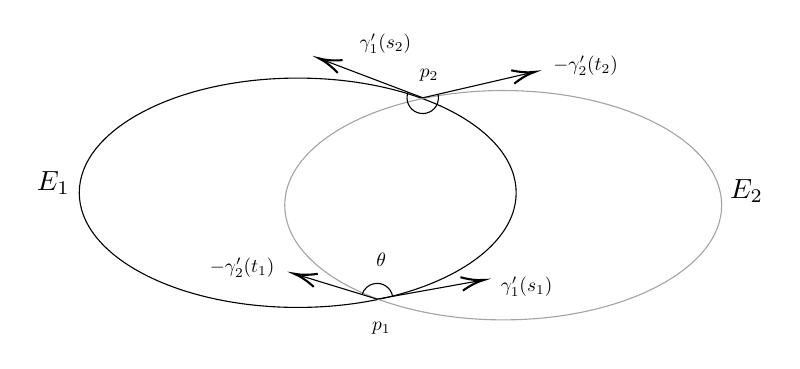
\begin{tikzpicture}[x=0.75pt,y=0.75pt,yscale=-1,xscale=1]
every edge quotes/.append style = {anchor=south, sloped}

%uncomment if require: \path (0,191); %set diagram left start at 0, and has height of 191

%Shape: Ellipse [id:dp10634347053631776] 
\draw   (68.5,97.75) .. controls (68.5,67.24) and (115.62,42.5) .. (173.75,42.5) .. controls (231.88,42.5) and (279,67.24) .. (279,97.75) .. controls (279,128.26) and (231.88,153) .. (173.75,153) .. controls (115.62,153) and (68.5,128.26) .. (68.5,97.75) -- cycle ;
%Shape: Ellipse [id:dp7816950476685691] 
\draw  [color={rgb, 255:red, 163; green, 163; blue, 163 }  ,draw opacity=1 ] (167.5,103.75) .. controls (167.5,73.24) and (214.62,48.5) .. (272.75,48.5) .. controls (330.88,48.5) and (378,73.24) .. (378,103.75) .. controls (378,134.26) and (330.88,159) .. (272.75,159) .. controls (214.62,159) and (167.5,134.26) .. (167.5,103.75) -- cycle ;
%Straight Lines [id:da36505632658461096] 
\draw    (234,52) -- (185.87,33.72) ;
\draw [shift={(184,33)}, rotate = 381.03999999999996] [color={rgb, 255:red, 0; green, 0; blue, 0 }  ][line width=0.75]    (10.93,-3.29) .. controls (6.95,-1.4) and (3.31,-0.3) .. (0,0) .. controls (3.31,0.3) and (6.95,1.4) .. (10.93,3.29)   ;

%Straight Lines [id:da357569598162492] 
\draw    (234,52) -- (286.05,39.95) ;
\draw [shift={(288,39.5)}, rotate = 526.97] [color={rgb, 255:red, 0; green, 0; blue, 0 }  ][line width=0.75]    (10.93,-3.29) .. controls (6.95,-1.4) and (3.31,-0.3) .. (0,0) .. controls (3.31,0.3) and (6.95,1.4) .. (10.93,3.29)   ;

%Straight Lines [id:da9574900886541131] 
\draw    (212,149) -- (173.91,137.34) ;
\draw [shift={(172,136.75)}, rotate = 377.03] [color={rgb, 255:red, 0; green, 0; blue, 0 }  ][line width=0.75]    (10.93,-3.29) .. controls (6.95,-1.4) and (3.31,-0.3) .. (0,0) .. controls (3.31,0.3) and (6.95,1.4) .. (10.93,3.29)   ;

%Straight Lines [id:da5801314237314061] 
\draw    (212,149) -- (261.53,140.1) ;
\draw [shift={(263.5,139.75)}, rotate = 529.8199999999999] [color={rgb, 255:red, 0; green, 0; blue, 0 }  ][line width=0.75]    (10.93,-3.29) .. controls (6.95,-1.4) and (3.31,-0.3) .. (0,0) .. controls (3.31,0.3) and (6.95,1.4) .. (10.93,3.29)   ;


% Text Node
\draw (216,26) node [scale=0.7]  {$\gamma _{1} '( s_{2})$};
% Text Node
\draw (312.5,36.5) node [scale=0.7]  {$-\gamma _{2} '( t_{2})$};
% Text Node
\draw (284,143) node [scale=0.7]  {$\gamma _{1} '( s_{1})$};
% Text Node
\draw (147,134) node [scale=0.7]  {$-\gamma _{2} '( t_{1})$};
% Text Node
\draw (214,163) node [scale=0.7]  {$p_{1}$};
% Text Node
\draw (237,41) node [scale=0.7]  {$p_{2}$};
% Text Node
\draw (56,93) node   {$E_{1}$};
% Text Node
\draw (390,97) node   {$E_{2}$};


\coordinate (O) at (212,149) ;
\coordinate (A) at (261.53,140.1) ;
\coordinate (B) at (173.91,137.34) ;

\coordinate (O2) at (234,52);
\coordinate (A2) at (185.87,33.72);
\coordinate (B2) at (286.05,39.95);

\draw (214,130) node [scale=0.7]  {$\theta$};

\draw pic[draw=black, -, angle eccentricity=1.2, angle radius=0.2cm]
{angle=A--O--B};

\draw pic[draw=black, -, angle eccentricity=1.2, angle radius=0.2cm]
{angle=A2--O2--B2};

\end{tikzpicture}

    \fautor
    \label{fig:ellipse_gamma}
\end{figure}

The following lemma states a relation between $s_1$ and $\Gamma_+(1,2)$

\begin{lema}\label{lema:lema_ellipse_angle}
	Let $\theta$ be the angle between $\gamma_1'(s_1)$ and $\gamma_2'(t_1)$ (counter-clockwise). Then, $\theta > \pi$ if, and only if $\Gamma_+(1,2)=s_1$.
\end{lema}

Instead of a formal proof of \autoref{lema:lema_ellipse_angle}, a graphical explanation using \autoref{fig:ellipse_gamma} is provided.


First, let us state some facts that can also be seen in \autoref{fig:ellipse_gamma}

\begin{itemize}
    \item $E_1 \cap E_2$ is convex and bounded by two arcs, one from each ellipse.
    \item Starting at any of the intersection points, one of the $E_1 \cap E_2$ arcs will be clockwise-oriented and the other counter-clockwise-oriented.
    \item The counter-clockwise-oriented arc starting at $\Gamma_+(1,2)$ is from $E_1$.
\end{itemize}


Let us assume that $p_1$ is the intersection point which is the opening angle $\Gamma_+(1,2)$. Then, the vectors $\gamma_1'(s_1)$ and $-\gamma_2'(t_1)$ are tangent to the $E_1 \cap E_2$ area at point $p_1$. Because of the convexity of $E_1 \cap E_2$, the angle between $\gamma_1'(s_1)$ and $-\gamma_2'(t_1)$ has to be less than or equal to $\pi$, therefore the angle between $\gamma_1'(s_1)$ and $-\gamma_2'(t_1)$ has to be greater than $\pi$, which is what \autoref{lema:lema_ellipse_angle} says. It is easy to see that the converse is also true assuming that $p_1$ is the point which determines the angle $\Gamma_-(1,2)$. 

Lastly, in \autoref{fig:ellipse_gamma}, it can be seen that if one point is classified as $\Gamma_+(1,2)$ the other will necessarily be classified as $\Gamma_-(1,2)$.
Computationally, this classification can be done taking the cross product of the two vectors and checking its signal, negative cross products imply an angle greater than $\pi$.



\end{apendicesenv}
% ---


% ----------------------------------------------------------
% Anexos
% ----------------------------------------------------------

% ---
% Inicia os anexos
% ---
%\begin{anexosenv}

%    \chapter{Páginas interessantes na Internet} 
%    \label{chapter:paginas-interessantes}
%    \begin{description}
 \item[\url{http://www.tex-br.org}] Página em português com diversos tutoriais e referências interessantes sobre \LaTeX;
 \item[\url{http://en.wikibooks.org/wiki/LaTeX}] Livro em formato \textit{wiki} gratuito sobre \LaTeX;
 \item[\url{http://tobi.oetiker.ch/lshort/lshort.pdf}] Ótimo tutorial sobre \LaTeX (possui versão em português \url{http://alfarrabio.di.uminho.pt/~albie/lshort/ptlshort.pdf}, mas a versão em inglês é a mais atual);
 \item[\url{http://code.google.com/p/abntex2/}] Página do abnTeX2, grupo que desenvolve os pacotes e classes em \LaTeX para as normas da ABNT, nos quais a classe \textit{icmc} foi baseada;
\item[\url{http://www.more.ufsc.br}] Página do Mecanismo On-line para Referências  (MORE) desenvolvido pela UFSC;
\item[\url{http://detexify.kirelabs.org/classify.html}] Página para recuperar o código de símbolos em \LaTeX a partir do desenho fornecido pelo usuário.
 \end{description}

%\end{anexosenv}
% ---

\end{document}